\documentclass[conference]{IEEEconf}
\IEEEoverridecommandlockouts
% The preceding line is only needed to identify funding in the first footnote. If that is unneeded, please comment it out.
\usepackage{cite}
\usepackage{amsmath,amssymb,amsfonts}
\usepackage{amsthm}
\usepackage{algorithm}
\usepackage{algorithmic}
\usepackage{graphicx}
\usepackage[hidelinks]{hyperref}
\usepackage{textcomp}
\usepackage{xcolor}
\def\BibTeX{{\rm B\kern-.05em{\sc i\kern-.025em b}\kern-.08em
    T\kern-.1667em\lower.7ex\hbox{E}\kern-.125emX}}

\DeclareMathOperator{\degr}{deg}     % degree operator: \degr(i)
\newcommand{\Ni}{\mathcal{N}}        % neighbor set: \Ni(i)
\newcommand{\CN}[2]{\Ni(#1)\cap\Ni(#2)} % common neighbors: \CN{i}{j}
\newcommand{\Nii}[1]{\Ni^{(2)}(#1)}  % 2-hop neighbors

\renewcommand{\algorithmicrequire}{\textbf{Input:}}
\renewcommand{\algorithmicensure}{\textbf{Output:}}

\newcommand{\xyu}[1]{\textcolor{magenta}{#1}}

\theoremstyle{plain}
\newtheorem{assumption}{Assumption}
\newtheorem{theorem}{Theorem} % Defines the 'theorem' environment
\newtheorem{lemma}{Lemma}     % Defines the 'lemma' environment
\newtheorem{definition}{Definition} % Defines the 'definition' environment
\newtheorem{example}{Example}
\newtheorem{remark}{Remark}

\title{\LARGE \bf
Distributed Control Framework for Connectivity Preservation and Collective Reconfiguration in Flow-Driven Robot Fleets}
\author{Prajjwal Dutta, Geoff Hollinger, and Xi Yu\\
%	{\small Department of Mechanical Engineering and Applied Mechanics} \\
%	University of Pennsylvania, Philadelphia, USA \\
%		\{xyureka,m.hsieh\}@seas.upenn.edu
%\thanks{*We gratefully acknowledge the support of ONR Award No. N00014-17-1-2690 and ARL DCIST CRA W911NF-17-2-0181.}
 \thanks{This work was supported by the NSF Awards 2322055 and 2529791.}
 \thanks{P. Dutta and X. Yu is with the School of Manufacturing Systems and Networks at Arizona State University (e-mail: \{pdutta9, xyu\}@asu.edu).
 G. Holinger is with the Department of Mechanical, Industrial, and Manufacturing Engineering at Oregon State University (e-mail: Geoff.Hollinger@oregonstate.edu).
}
 }

\begin{document}

% \title{Decentralized Connectivity-Aware Control for Autonomous Underwater Vehicles under Environmental Disturbances*\\
% \thanks{This Project is funded by NSF Grant}
% }

% \author{\IEEEauthorblockN{1\textsuperscript{st} Prajjwal Dutta}
% \IEEEauthorblockA{\textit{School of Manufacturing Systems and Networks} \\
% \textit{Arizona State University}\\
% Tempe, AZ \\
% pdutta9@asu.edu}
% \and
% \IEEEauthorblockN{2\textsuperscript{nd} Geoff Hollinger}
% \IEEEauthorblockA{\textit{College of Engineering} \\
% \textit{Oregon State University}\\
% Corvallis, OR  \\
% Geoff.Hollinger@oregonstate.edu}
% \and
% \IEEEauthorblockN{3\textsuperscript{rd} Xi Yu}
% \IEEEauthorblockA{\textit{School of Manufacturing Systems and Networks} \\
% \textit{Arizona State University}\\
% Tempe, AZ \\
% xyu@asu.edu}
% }

\maketitle

\begin{abstract}
% Autonomous underwater vehicles (AUVs) deployed in under-ice and flow-disturbed environments must preserve network connectivity despite limited acoustic communication, environmental disturbances, and the absence of centralized supervision. Existing strategies often depend on centralized spectral methods or precomputed spanning trees, which require global information and are ill-suited for bandwidth- and energy-constrained deployments. This paper presents a decentralized framework that integrates distributed critical-edge detection with local pruning, recouping, and rewiring, combined with decentralized Control Lyapunov Function and Control Barrier Function (CLF--CBF) quadratic programs. Each robot enforces CBF constraints with respect to all neighbors, ensuring safety and connectivity, while the graph layer dynamically reduces redundancy by identifying and restructuring non-critical links. A physics-informed underwater environment model with drag, vortices, buoyancy, and turbulence is used to evaluate performance. Simulation results show that the proposed approach preserves connectivity while reducing redundant edges, achieving goal-seeking performance comparable to centralized methods, and significantly outperforming uncontrolled random motion. The results demonstrate the potential of decentralized connectivity-aware control for scalable, resilient AUV swarms operating in challenging sub-ice environments.
We study the deployment of underwater robot fleets in large, flow dominated environments where localization is denied, communication is limited, and energy is scarce. The robots need to travel long distances, detect emerging targets, and stay connected using only local information. To meet these challenges we design a distributed framework that exploits natural drift and activates control only when required. The method begins with the robots deployed as a fully connected network. Using minimal information exchange, each robot prunes non-critical edges, producing a sparse and tree like structure that spans the entire team. Upon this structure we construct a distributed control Lyapunov function–control barrier function (CLF–CBF) framework. Each robot enforces barrier constraints to maintain the necessary connections, while redundant links are discarded when alternative paths emerge. When a target is discovered, this framework ensures the detecting robot attends the target, while the team reconfigures to provide a connected formation. This approach guarantees long term connectivity with very low control effort, and enables collective response to dynamic tasks. Simulations validates the framework and demonstrates that it yields spanning structures that converge toward a minimum spanning tree over time, highlighting both its efficiency and robustness under realistic underwater conditions.
\end{abstract}

% \begin{IEEEkeywords}
% Decentralized control, Connectivity maintenance, Barrier functions (CBFs), Lyapunov functions (CLFs), autonomous underwater vehicles (AUVs), Brownian motion, Underwater modeling.
% \end{IEEEkeywords}

\section{Introduction}

We are interested in deploying a fleet of underwater robots into large-scale, challenging environments such as the deep ocean and under-ice cavities, where localization is denied, communication bandwidth is limited, and the environment is dominated by dynamic flows and eddies \cite{muto2024}. 
These robots must traverse long distances on limited energy budgets, discover emerging regions of interest, sample the environment, and relay data, all while relying on intermittent and bandwidth-limited communication \cite{schiel2024chirps, schiel2024role}.

The central challenge is to design strategies that enable the fleet to (i) expend minimal control effort while traveling long distances and completing complex tasks, (ii) efficiently cover a large spatial domain to discover emerging targets while maintaining network connectivity, and (iii) realize a globally connected configuration using only localized information and limited communication.

% Exploring sub-ice ocean cavities is critical for understanding glacial melt and predicting global sea-level rise. These extreme environments are among the most challenging places for autonomous systems: they are remote, shielded from satellite navigation, and deny radio or Global Positioning System (GPS) access. Communication is limited to low-bandwidth, high-latency acoustic signaling, which is easily disrupted by obstacles, multipath effects, and flow dynamics. In such conditions, relying on a central command structure is infeasible. Instead, autonomous underwater vehicles (AUVs) must coordinate in a \textit{fully decentralized} manner, exchanging minimal information with local neighbors while ensuring that the overall fleet remains connected.  

% Maintaining connectivity in these scenarios is non-trivial. Sparse and intermittent communication, combined with environmental disturbances, can fragment the network. At the same time, enforcing all possible links leads to dense communication graphs that waste energy, increase interference, and constrain mobility. What is needed is a distributed strategy that preserves only the essential edges required for global connectivity while enabling each agent to make local decisions that remain robust to flow and communication uncertainty.  

% The mothership project takes on this challenge by deploying a mothership AUV that releases swarms of low-cost passenger robots into under-ice cavities. These agents must self-organize, maintain sparse but resilient communication structures, and adapt to environmental disturbances without centralized supervision. This paper contributes to this vision by developing a framework for \textit{connectivity-aware coordination} that couples graph-theoretic sparsification with local control under flow disturbances.  

% The main contributions of this paper are as follows:
% \begin{enumerate}
%     \item Critical edge detection, pruning, and recouping. We extend distributed bridge-detection methods to identify critical links, prune redundant edges using a redundancy-aware priority metric, and recoup connectivity when pruning risks of fragmentation.
%     \item Decentralized rewiring optimization. Each agent evaluates $k$-hop alternatives and performs safe local rewiring to improve efficiency while preserving global connectivity.
%     \item Integration of Control Lyapunov Function (CLF) and Control Barrier Function (CBF) based controllers into evolving graphs. All robots solve local Quadratic Programs (QPs) that combine CLFs for goal convergence or relay maintenance with CBFs for safety and connectivity, applied only to the evolving pruned/optimized edge set.
% \end{enumerate}

% We validate the proposed framework in a physics-informed underwater flow-field environment that models drag, vortices, buoyancy, and stochastic disturbances, demonstrating its robustness and direct relevance to large-scale exploration under ice.

Our proposed approach is to deploy the robots together and then allow them to drift with the prevailing flow as much as possible. Control effort is only applied when it is necessary. This includes situations when the robots risk drifting outside a prescribed region or when they risk losing connectivity. In this way the formation disperses while staying connected, and the group can also reconfigure when a new target location is discovered or generated \cite{butler2025}. This strategy is bold, but it is supported by recent progress. Previous work has shown that surface vehicles can drift with the flow while using minimal control to remain in gyre like structures \cite{wei2019}, or track the periodicity of revisits via intermittent control triggered by prescribed conditions \cite{knizhnik2022}. In addition, broadly adopted models describe the uncontrolled motion of objects in water as drift combined with Brownian type diffusion \cite{taylor1922, okubo1971, majda1999}, which align with observation on underwater robots \cite{berlinger2021, quattrini2023}. This indicates that our fleet will approximately follow the main direction of the flow while also dispersing stochastically.

Although dispersion promotes coverage of large task spaces, two challenges remain open. The first is how to maintain connectivity. The second is how to enable reconfiguration around targets while working with strict energy budgets and unreliable communication that cannot support centralized control. Prior work on connectivity maintenance and target surrounding has emphasized the importance of graph theoretic methods \cite{olfati2007,dimartino2006}. Control barrier functions (CBFs) have received attention for their energy efficiency in this setting. For example, CBFs have been applied to the Fiedler value of the network graph in order to maintain connectivity \cite{capelli2020}. This approach is effective but it requires centralized and computationally expensive eigenvalue calculations. Other work has applied distributed CBF formulations that keep robots pairwise within communication range \cite{sabattini2013,capelli2021}. More recently, a hybrid framework was introduced that combines distributed CBFs with a graph theoretic tool, where each robot interacts only with a limited set of neighbors defined by a minimum spanning tree (MST) \cite{yang2023}. This solution is promising since each robot only applies CBF to itself and to selected neighbors, but it still requires generating a minimum spanning tree that depends on global information.

In our case a feasible framework must combine two ingredients. The first is a distributed neighbor selection strategy so that each robot chooses a limited set of neighbors to remain within communication range. The second is a local control law applied only to these neighbors. Together these two features must guarantee global connectivity while minimizing control effort. Work on spanning trees has shown that distributed verification methods exist, but the actual construction of a minimum spanning tree is classically centralized \cite{boruvka1926, kruskal1956, prim1957}. Progress in fully distributed protocol for exact MST construction \cite{gallager1983, awerbuch1987} remain communication-intensive. As a result, several approximate or near-optimal distributed methods have been proposed, but they do not achieve exact solutions \cite{khan2008}.

We take advantage of two physical features of our problem. First, the robots are deployed together, and the initial configuration forms a fully connected graph. Second, the purpose of a spanning tree is to reduce long range connections. A robot should drop links to distant neighbors whenever a closer neighbor can maintain connectivity at lower control cost. Recent progress \cite{venkateswaran2024} has also shown that robots can verify whether an edge is critical, meaning that breaking it would break the network connectivity, using distributed procedures that rely only on very limited data sharing. Based on these observations we propose a distributed method that requires very little information exchange. Each robot shares only a list of its neighbor indices. With this limited data the robots identify and prune edges that are not critical to connectivity. The result is a sparse and tree-like structure that spans the entire network. Once this structure is established, we construct a distributed control Lyapunov function–control barrier function (CLF–CBF) framework upon it. Each robot maintains only the necessary connections by enforcing CBF constraints, and redundant links are pruned whenever new edges provide alternative paths. When a target is detected, the framework drives the robot that discovers it toward the target, while the rest of the team reconfigures to form a supporting network from the bottom up. As a result, the team preserves connectivity, expands to maintain coverage, and collectively shifts toward the target location.

Simulations demonstrate that this method can efficiently attend to emerging targets in different regions of the environment while keeping the network connected. Over deployment time the spanning structure produced by this distributed pruning strategy converges toward a minimum spanning tree. This shows both its long term efficiency and its robustness in flow dominated and resource constrained conditions.

This paper is organized as follows. Sec.~\ref{sec:prob} introduces the problem. Sec.~\ref{sec:method} presents our two-fold control framework. Sec.~\ref{sec:result} demonstrates the results of the proposed method via simulated examples. Sec.~\ref{sec:conclusion} concluded this work. % begins by introducing the background and problem formulation, outlining the assumptions on communication, dispersion, and formulating the problem statement. It then presents the proposed methodology, starting with distributed edge detection and pruning, and extending to a decentralized CLF--CBF control framework built on the resulting sparse network backbone. The simulation setup and results are described next, including comparisons with centralized baselines and MST benchmarks. The paper concludes with a discussion of key findings and potential directions for future work.

%\section{Literature Review}

% Preservation of connectivity in robot teams has been studied through several approaches. Classic methods maintain global connectivity through spectral analysis, for example, by ensuring a positive lower bound on the algebraic connectivity of the graph (the second smallest Laplacian eigenvalue). These techniques provide elegant guarantees, but often assume global knowledge or centralized computation, which is not suited to bandwidth and energy-constrained deployments. A foundational survey of distributed coordination and consensus is a stepping stone to connectivity control \cite{1}. 

% Another widely used approach is based on CBFs, which enforce safety-critical constraints in real time via QPs. CBFs are effective for collision avoidance and communication range maintenance \cite{2}. Safety constraints must be enforced for all agents within interaction range to guarantee collision-free operation. Connectivity preservation can also be encoded as a barrier function.

% From the graph-theoretic side, several algorithms have been proposed for detecting critical edges, or bridges, in undirected networks. Yang, Lyu, and Luo revisited minimally constrained multi-robot coordination with explicit line-of-sight connectivity maintenance \cite{3}. Although this effectively preserves a minimal spanning structure, it is fundamentally centralized, as the spanning tree is computed globally and broadcast to the team. Other centralized approaches exploit the algebraic connectivity of the Laplacian. De Gennaro and Jadbabaie proposed gradient-based strategies to increase the second smallest eigenvalue ($\lambda_2$) \cite{4}, and later works incorporated CBFs into $\lambda_2$-based formulations \cite{5}. However, all of these methods depend on globally shared spectral information, making them difficult to implement in resource constrained multi-robot settings.  

% In contrast, decentralized strategies rely only on local neighbor information. Sabattini introduced decentralized rules for reconfigurable coordination based on local connectivity and collision avoidance specifications \cite{6}, and subsequent work extended CBF formulations to account for delays and disturbances, providing decentralized controllers that maintain safety under imperfect communication \cite{7}. These approaches improve scalability but typically stop at enforcing pairwise connectivity or safety constraints; they do not leverage critical-edge detection to prune redundancy or restructure the network dynamically. Our work adopts distributed critical edge detection as a baseline, building on the method presented in \cite{8}. We extend this foundation by coupling pruning, recouping, and rewiring with decentralized CLF-CBF controllers. This represents a shift from centralized spanning tree or spectral methods toward a fully decentralized, connectivity-aware framework.

% In underwater multi-robot systems, dispersal and spreading behaviors have been studied as mechanisms to improve coverage and robustness in exploration tasks. For example, Berlinger demonstrated that implicit coordination strategies allow AUV groups to maintain distributed formations in three-dimensional underwater environments, enabling sampling and mapping under visibility constraints \cite{9}. These studies show that dispersive motion is both natural and often beneficial for underwater collectives, but they generally do not address connectivity preservation under acoustic communication limits. Furthermore, environmental disturbances such as currents and drag can intensify dispersive effects, complicating coordination and highlighting the difficulty of maintaining reliable inter-vehicle communication in practice.

% So, the underwater and sub-ice robotics literature emphasizes the operational constraints that motivate decentralized solutions. Acoustic communication links are characterized by low bandwidth and high latency, and are easily disrupted by multipath interference or occlusions \cite{9}. Moreover, AUV motion is perturbed by external currents, vortices, and drag forces, which degrade control accuracy and increase energy consumption \cite{10}. These challenges have been highlighted not only in surveys of underwater communication and control, but also in recent modeling studies of AUV fleets under environmental disturbances, including our prior work on connectivity-aware coordination and underwater flow-field simulation \cite{11}. In such conditions, centralized strategies are impractical, and robots must rely on neighbor based coordination.

% In summary, existing approaches either maintain connectivity, assuming a centrally computed spanning structure, or detect critical edges without integrating them into dynamic control. The contribution of this work is to unify these strands by combining distributed critical edge detection with pruning and recouping of redundant links, enabling local rewiring optimization, and embedding them into a decentralized CLF-CBF controller. This shift from centralized, precomputed structures, as demonstrated in \cite{3}, to a fully decentralized, neighbor-only implementation constitutes the key conceptual advance of our approach.

\section{Background and Problem Formulation}\label{sec:prob}

We now formalize the problem. This section introduces the robot dynamics model, states the assumptions, defines the graph-theoretic notation, and presents the formal problem statement.
\subsection{Advection-diffusion model \cite{taylor1922, okubo1971, majda1999}}
%\xyu{Edit the notation to align with your notations on the flow field.}

We model a fleet of $N$ robots operating in $\mathbb{R}^n$ (with $n=2$, used for visualization in our simulations) released together in the water, their collective motion can be decomposed into a drift component induced by an ambient flow field and a stochastic dispersion component due to unexpected turbulence and small perturbations. Let $x_i(t) \in \mathbb{R}^n$ denote the position of the $i$-th robot at time $t$, where $i\in \{1,2,...,N\}$, and let  
\[
\bar{x}(t) = \frac{1}{N} \sum_{i=1}^N x_i(t)
\]  
be the center of mass of the group. 

The evolution of the center of mass is governed primarily by the advective flow field, i.e.,  
\[
\dot{\bar{x}}(t) \approx f_{\text{flow}}(\bar{x}(t),t),
\]  
where $f_{\text{flow}}$ is the background velocity field. Each individual object then deviates from $\bar{x}(t)$ due to unresolved small-scale turbulence and fluctuations, which can be modeled as Brownian motion:  
\begin{equation}
\begin{gathered}
    dx_i(t) = (f_{\text{flow}}(x_i(t), t) + v_i(t)) dt + \sigma_{\text{diff}} dW_i(t) \\
    \dot{v}_i(t) = u_i(t) - \gamma v_i(t)
\end{gathered}
\end{equation}
\noindent where $v_i(t) \in \mathbb{R}^n$ is the velocity of each individual robot, $u_i(t) \in \mathbb{R}^n$ is the thrust, $\gamma > 0$ is a velocity damping factor, and $W_i(t)$ is a Wiener process capturing diffusion (with intensity $\sigma_{\text{diff}}$).

Thus the group drifts together with the flow through the motion of $\bar{x}(t)$, while individuals spread stochastically around the drifting center due to the independent diffusion terms.

As an example, the flow field is a base current plus a spatially varying swirl:
\begin{equation*}
f_{\text{flow}}(x,t) = v_{\text{base}}(t) + A_{\text{swirl}}
\begin{bmatrix}
    \sin \! \left( \tfrac{x_2 + t}{s_{\text{swirl}}} \right) \\
    \cos \! \left( \tfrac{x_1 + 0.3t}{s_{\text{swirl}}} \right)
\end{bmatrix}
\end{equation*}
For two robots $i$ and $j$, the flow difference is generally nonzero when $x_{i} \neq x_{j}$:
\begin{equation*}
f_{\text{flow}}(x_i, t) - f_{\text{flow}}(x_j, t) = A_{\text{swirl}}
\left[ \begin{smallmatrix}
    \sin \! \left( \frac{x_{i,2} + t}{s_{\text{swirl}}} \right) - \sin \! \left( \frac{x_{j,2} + t}{s_{\text{swirl}}} \right) \\
    \cos \! \left( \frac{x_{i,1} + 0.3t}{s_{\text{swirl}}} \right) - \cos \! \left( \frac{x_{j,1} + 0.3t}{s_{\text{swirl}}} \right)
\end{smallmatrix} \right] \neq 0
\end{equation*}

We assume that the ambient flow is spatially smooth and its differential drift is bounded:
$$
\|f_{\text{flow}}(x_i, t) - f_{\text{flow}}(x_j, t)\| \le L_f \|x_i - x_j\|, \quad \forall x_i, x_j, \quad \forall t \ge 0.
$$
If the flow were spatially uniform, it would cancel in the relative dynamics. This assumption explicitly captures the non-uniform, spatially varying regime by bounding how much the flow can differ across inter-robot distances. For the swirl flow field, one can take this flow as globally lipschitz in $x$ with a lipschitz constant $L_f \approx A_{\text{swirl}} / s_{\text{swirl}}$.

\subsection{Control-affine model}
For controller synthesis and theoretical analysis, we now abstract the above simulation dynamics into a compact control-affine model on $x_i$:
\begin{equation}\label{eq:adv-dif}
\dot{x}_i(t) = f_{\text{flow}}(x_i(t),t) + u_i(t) + d_i(t), \quad \|d_i(t)\|\le \bar d.
\end{equation}

With the control input $u_i(t)$ set to zero throughout the deployment time window, the robots will be passively advected by the background flow while gradually dispersing due to stochastic perturbations. Here the unmodeled effects of drag, turbulance and stochastic perturbations are captured by a bounded disturbance term:

$$\|d_i(t)\| \le \bar{d}, \quad \forall i \in \mathcal{V}, \quad \forall t \ge 0. $$
This term corresponds to the combined effect of Brownian motion, transient velocity dynamics, and model uncertainties that are abstracted away in the reduced model.

We present two different dynamics descriptions because they serve different purposes. The advection-diffusion model supports physical interpretation and simulation realism, while the control affine model is used to controller design and theoretical analysis in section \ref{sec:method}. The flow term is evaluated at each robot's position, so it is not a common input that is identical for all the robots in relative coordinates ${z_{ij}} = {x_i} - {x_j}$,
\begin{equation*}
    \dot{z}_{ij} = (f_{\text{flow}}(x_i, t) - f_{\text{flow}}(x_j, t)) + (u_i - u_j) + (d_i - d_j)
\end{equation*}
So, the flow contribution cancels only in the special case of spatially uniform flow. In our setting, spatial variation of $f_{flow}$ is explicitly bounded (assumption), which is quantity that enters the connectivity and invariance analysis.

The time derivative of the squared inter-robot distance can be written as
\begin{equation*}
    \dot{z}_{ij}^2 = 2{z}_{ij}^\top \Big( \big( f_{\text{flow}}(x_i,t) - f_{\text{flow}}(x_j,t) \big) + (v_i - v_j) \Big)
\end{equation*}
This expression makes explicit that the flow contributes through the \textit{difference term} $f_{\text{flow}}(x_i,t)-f_{\text{flow}}(x_j,t)$.


Notice that the choice of a two-dimensional environment is made solely for ease of visualization. The developed method is dimension-agnostic and extends directly to three-dimensional settings.

\subsection{Assumptions on communication, control and connectivity}
\label{subsec:assumptions}

\begin{assumption}
\label{ass:A1}
For all robots $i$ and all $t\ge 0$, the inputs are bounded and the control authority dominates the worst case advection  and disturbance over the communication range:
\begin{equation}
\|u_i(t)\| \le u_{\max}
\label{eq:A1}
\end{equation}
\begin{equation}
u_{\max} \;>\; \bar d + L_f R_{\max}
\label{eq:A2}
\end{equation}
\end{assumption}

\begin{assumption}
\label{ass:A2}
The minimum separation distance is strictly smaller than the communication range with a nonzero buffer:
\begin{equation}
d_{\min} \;<\; R_{\max} - \varepsilon
\label{eq:A3}
\end{equation}
for some margin $\varepsilon>0$.
\end{assumption}

\begin{assumption}
\label{ass:A3}
At time $t$, the communication network is an undirected disk graph $\mathcal{G}_t=(\mathcal{V},\mathcal{E}_t)$ with range $R_{\max}>0$:
\begin{equation}
(i,j)\in\mathcal{E}_t \quad \Longleftrightarrow \quad \|x_i(t)-x_j(t)\|\le R_{\max}.
\label{eq:disk_graph}
\end{equation}
Each robot $i$ communicates only with its neighbors in its neighbouring set
\begin{equation}
\mathcal{N}_i(t) \triangleq \{\, j\in\mathcal{V} : \|x_i(t)-x_j(t)\|\le R_{\max}\,\},
\label{eq:neighbors}
\end{equation}
using only neighbor communication without any central coordination. Each robot has a unique identifier to index neighbor messages consistently. The initial graph $\mathcal{G}_0$ is connected.
\end{assumption}

\begin{assumption}
\label{ass:A4}
    During the distributed consensus/pruning phases, $\mathcal{G}_{topo}$ remains connected and varies slowly enough that information can propagate across the network and the required consensus iterations converge before $\mathcal{G}_{topo}$ changes significantly.
\end{assumption}

%We model these $N$ robots indexed by $i \in \mathcal{V}=\{1,\dots,N\}$, each with planar position $x_i \in \mathbb{R}^2$ and bounded control input $u_i \in \mathbb{R}^2$, with $\|u_i\|\leq u_{\max}$. Robots follow single-integrator dynamics 
%\[
%\dot{x}_i = u_i,
%\] 
%and a minimum pairwise separation distance $d_{\min}>0$ must be maintained to avoid collisions.  

%The communication network is described by the standard disk model with nominal range $R_{\max}>0$. At time $t$, an undirected edge $(i,j)$ exists between robots $i$ and $j$ if $\|x_i(t)-x_j(t)\| \leq R_{\max}$. The resulting network is represented by the undirected graph $\mathcal{G}_t = (\mathcal{V},\mathcal{E}_t)$, where the vertex set $\mathcal{V}$ corresponds to robots and the edge set $\mathcal{E}_t$ encodes pairwise communication links. The neighborhood of robot $i$ is defined as  
%\[
%\Ni(i) = \{ j \in \mathcal{V} : \|x_i(t)-x_j(t)\| \leq R_{\max} \},
%\]  
%so that agent $i$ observes relative states and exchanges messages only with robots in $\Ni(i)$. We denote the degree of node $i$ as $\deg(i)=|\Ni(i)|$. The set of common neighbors of two nodes $i,j$ is $\CN{i}{j}$, and the two-hop neighbors of $i$ are $\Nii{i} = \{k \in \mathcal{V} : \exists j \in \Ni(i) \text{ with } k \in \Ni(j)\}$. The initial communication graph $\mathcal{G}_0=(\mathcal{V},\mathcal{E}_0)$ is assumed to be connected. Connectivity is defined in the standard graph-theoretic sense: the graph $\mathcal{G}_t$ is connected if, for every pair $i,j \in \mathcal{V}$, there exists a path in $\mathcal{E}_t$ linking them. No global positions, centralized maps, or spectral information are assumed to be available.  

\subsection{Problem Statement}
\label{subsec:problem_statement}

Consider the multi-robot system introduced above with dynamics~\eqref{eq:adv-dif} and communication model~\eqref{eq:disk_graph}--\eqref{eq:neighbors}. The robots are advected by a spatially varying ambient flow field $f_{\text{flow}}(x,t)$ and are subject to bounded disturbances $d_i(t)$, which together induce natural dispersion. While this dispersion promotes exploration, it can also stretch inter-robot distances and break communication links.

Let $\mathcal{G}_t=(\mathcal{V},\mathcal{E}_t)$ denote the physical disk graph induced by the range $R_{\max}$ (Assumption~\ref{ass:A3}). During the mission, robots may intentionally sparsify the network by maintaining a time-varying coordination subgraph $\mathcal{G}_{\mathrm{topo}}(t)=(\mathcal{V},\mathcal{E}_{\mathrm{topo}}(t))$ with $\mathcal{E}_{\mathrm{topo}}(t)\subseteq \mathcal{E}_t$.

We formalize the hard safety/connectivity requirements using the constraint sets
\begin{align*}
\mathcal{C}_{\mathrm{safe}} &\triangleq \Big\{x\in(\mathbb{R}^n)^N : \|x_i-x_j\|\ge d_{\min},\;\forall i\neq j\Big\},\\
\mathcal{C}_{\mathrm{conn}}(\mathcal{E}) &\triangleq \Big\{x\in(\mathbb{R}^n)^N : \|x_i-x_j\|\le R_{\max},\;\forall (i,j)\in\mathcal{E}\Big\},
\end{align*}
and the admissible input set $\mathcal{U}\triangleq\{(u_1,\dots,u_N):\|u_i\|\le u_{\max}\;\forall i\}$ (Assumption~\ref{ass:A1}).

Targets (locations of interest) are not known a priori and are detected only when an agent enters its sensing footprint. During exploration (no detection), the team should drift with $f_{\text{flow}}$ while remaining connected and reducing communication redundancy. Upon target detection, a subset of agents should initiate goal-seeking behavior while the remaining agents act as relays so that end-to-end connectivity across the fleet is preserved.

Each agent $i$ has access only to local information: (i)~its own state $x_i$; (ii)~relative states $\{x_j-x_i\}_{j\in\mathcal{N}_i(t)}$ and messages from one-hop neighbors; and (iii)~local graph quantities, like two hop connection, are computable through neighbor exchanges. We denote this information set by $\mathcal{I}_i(t)$. No centralized computation, global maps, spanning trees, or spectral quantities are assumed.

\noindent\textbf{Distributed connectivity-preserving control with topology sparsification.}
Design distributed policies consisting of (i)~a feedback control law $u_i(t)=\kappa_i(\mathcal{I}_i(t))$ for each agent and (ii)~a distributed pruning/maintenance rule that generates $\mathcal{E}_{\mathrm{topo}}(t)\subseteq\mathcal{E}_t$, using only local information, such that for all $t\ge 0$:
\begin{enumerate}
    \item  $x(t)\in\mathcal{C}_{\mathrm{safe}}$ and $x(t)\in\mathcal{C}_{\mathrm{conn}}(\mathcal{E}_{\mathrm{topo}}(t))$, and the maintained graph $\mathcal{G}_{\mathrm{topo}}(t)$ remains connected.
    \item The controller exploits advection and uses minimal actuation (e.g., keeps $\|u_i(t)\|$ small and activates control only when constraints would be violated).
    \item The team spreads for coverage during exploration and, upon target detection, reconfigures so that designated agents make progress toward the target while relays preserve end-to-end connectivity.
\end{enumerate}

The proposed framework in Sec.~\ref{sec:method} provides a fully distributed realization of these objectives via distributed topology sparsification and decentralized CLF--CBF control.


%\subsection{Problem Statement}

%Consider the robots and communication network introduced in the previous section.  
%The robots are advected by the background flow field $f_{\text{flow}}$ and subject to stochastic perturbations that induce dispersion (as introduce in eq.~\eqref{eq:adv-dif}).  
%This natural dispersion promotes exploration but risks breaking connectivity.  
%Locations of interest are not known a priori and are only detected when an agent enters its sensing footprint.  
%During exploration phases (when no target is detected), the team drifts with %$f_{\text{flow}}$ while maintaining connectivity and sparsifying the communication graph.  
%When a target is detected, a local subset of agents initiates goal-seeking behavior while the remaining agents act as relays to preserve end-to-end connectivity across the fleet.  

%Each agent $i$ has access to:  
%(i) its own state $x_i$;  
%(ii) relative states $\{x_j - x_i\}_{j \in \Ni(i)}$ and messages received from neighbors; and  
%(iii) local graph quantities that can be computed through neighbor exchanges, such as two-hop information.  
%No centralized computation, global identifiers beyond local exchanges, globally shared maps, spanning trees, or spectral quantities (e.g., eigenvalues) are assumed.  

%The problem is therefore to design a \textbf{distributed control framework} that satisfies the following objectives:  

%\begin{enumerate}
 %   \item \textbf{Connectivity preservation:} ensure that the communication graph $\mathcal{G}_t$ remains connected for all $t$.  
  %  \item \textbf{Energy efficiency:} leverage flow advection and activate inputs only when necessary.  
  %  \item \textbf{Collective reconfiguration:} enable the team to spread out for coverage during exploration and shift toward newly discovered targets, while maintaining connectivity and collision avoidance.  
%\end{enumerate}

%The solution must rely exclusively on local relative information and distributed exchanges, without requiring any centralized solver or globally shared information.   


% Given:
% (i) an initially connected, range-induced graph $G_0=(V,E_0)$ with radius $R_{\max}$;
% (ii) single-integrator agents evolving under an unknown flow field with bounded disturbances as above;
% (iii) a safety distance $d_{\min}$ and input bound $u_{\max}$; and
% (iv) neighbor-only information exchanges,

% design fully decentralized, per-agent policies that, at each timestep:
% (a) classify edges using only local exchanges and prune non-critical links while guaranteeing that $G_t$ remains connected and no node is isolated;
% (b) perform local recouping within 1–2 hops to preserve efficiency and robustness against flow-induced drift and intermittent line-of-sight breaks; and
% (c) compute control inputs $u_i$ via decentralized CLF–CBF that ensure safety and connectivity at all times and activate goal-seeking upon target detection,

% so that the fleet uses limited energy (minimizes control effort), spreads out to cover space yet stays connected, and can reshuffle formation to send one or more robots to attend task locations while preserving end-to-end connectivity, all under environmental disturbances and without centralized supervision.

\section{Methodology}

\label{sec:method}

Our method proposes a fully distributed framework with a combination of two layers. The control layer enforces safety and a set of communication edges under spatially varying flow using control barrier functions (CBFs). The graph layer uses neighbor to neighbor message passing to identify connectivity network and prune non-essential edges without centralized computation. Building on this a CLF CBF controller activates goal seeking behavior while maintaining safety and end to end connectivity. Each component is detailed in the following subsections.

We first establish if certain CBF constraints are enforced, then safety and selected communication links remain satisfied for all time.

%Our method has two components. First, we identify a sparse critical communication structure by pruning non-essential edges.  
%Then, we apply a distributed CLF-CBF framework on this structure to preserve connectivity and enable target-driven reconfiguration. Each component is detailed in the following subsections. 

\begin{theorem}[Invariance of safety and connectivity]
\label{thm:robust-invariance}
Consider the control-affine multi-robot model \eqref{eq:adv-dif} operating over the communication model \eqref{eq:disk_graph}--\eqref{eq:neighbors}. Let Assumptions~\ref{ass:A1}--\ref{ass:A3} hold, and as mentioned in sec \ref{sec:prob}-A and \ref{sec:prob}-B, we consider the flow field satisfies the spatial smoothness bound
\(
\|f_{\text{flow}}(x_i,t)-f_{\text{flow}}(x_j,t)\|\le L_f\|x_i-x_j\|
\)
for all $x_i,x_j$ and all $t\ge 0$, and disturbances satisfy $\|d_i(t)\|\le \bar d$.
For any ordered pair $(i,j)$, define the relative position and distance
\[
z_{ij} \triangleq x_i-x_j,\qquad r_{ij}\triangleq \|z_{ij}\|.
\]

Fix two edge index sets:
(i) a \emph{safety-enforced} set $\mathcal{E}_s\subseteq \mathcal{V}\times\mathcal{V}$, and
(ii) a \emph{connectivity-enforced} set $\mathcal{E}_c \subseteq \mathcal{E}_0$.
Define the pairwise barrier functions
\begin{align}
h^{\mathrm{safe}}_{ij}(x) &\triangleq r_{ij}^2 - d_{\min}^2,
\label{eq:h_safe}\\
h^{\mathrm{conn}}_{ij}(x) &\triangleq R_{\max}^2 - r_{ij}^2.
\label{eq:h_conn}
\end{align}
Let $\alpha_s,\alpha_c:\mathbb{R}\to\mathbb{R}$ be extended class-$\mathcal{K}$ functions.

Suppose that for all $t\ge 0$ the applied controls satisfy $\|u_i(t)\|\le u_{\max}$ and, for every $(i,j)\in \mathcal{E}_s$, the \emph{robust safety CBF inequality}
\begin{equation}
{
2 z_{ij}^\top (u_i-u_j)\ \ge\ 2L_f r_{ij}^2 + 4\bar d\, r_{ij}\ -\ \alpha_s\!\big(h^{\mathrm{safe}}_{ij}(x)\big)
}
\label{eq:robust_safe_cbf}
\end{equation}
and for every $(i,j)\in \mathcal{E}_c$, the \emph{robust connectivity CBF inequality}
\begin{equation}
{
2 z_{ij}^\top (u_i-u_j)\ \le\ \alpha_c\!\big(h^{\mathrm{conn}}_{ij}(x)\big)\ -\ 2L_f r_{ij}^2 - 4\bar d\, r_{ij}.
}
\label{eq:robust_conn_cbf}
\end{equation}

Then the set
\begin{equation}
\label{eq:overall_safe_set}
\begin{aligned}
\mathcal{S}\triangleq\;
&\left(\bigcap_{(i,j)\in \mathcal{E}_s}
\left\{x:\ h^{\mathrm{safe}}_{ij}(x)\ge 0\right\}\right) \\
&\cap
\left(\bigcap_{(i,j)\in \mathcal{E}_c}
\left\{x:\ h^{\mathrm{conn}}_{ij}(x)\ge 0\right\}\right)
\end{aligned}
\end{equation}

is forward invariant for the closed-loop system. In particular, if initially
$h^{\mathrm{safe}}_{ij}(x(0))\ge 0$ for all $(i,j)\in\mathcal{E}_s$ and
$h^{\mathrm{conn}}_{ij}(x(0))\ge 0$ for all $(i,j)\in\mathcal{E}_c$,
then for all $t\ge 0$,
\begin{align}
\|x_i(t)-x_j(t)\| &\ge d_{\min}, &&\forall (i,j)\in \mathcal{E}_s,
\label{eq:safety_invariance}\\
\|x_i(t)-x_j(t)\| &\le R_{\max}, &&\forall (i,j)\in \mathcal{E}_c.
\label{eq:conn_invariance}
\end{align}
\end{theorem}

\begin{proof}
Fix any pair $(i,j)$. For compactness write $z \triangleq z_{ij}=x_i-x_j$, $r\triangleq \|z\|$, and denote
\[
\begin{aligned}
\Delta f_{ij}(t) &\triangleq f_{\text{flow}}(x_i,t)-f_{\text{flow}}(x_j,t),\\
\Delta d_{ij}(t) &\triangleq d_i(t)-d_j(t)
\end{aligned}
\]
From \eqref{eq:adv-dif}, the relative dynamics are
\begin{equation}
\dot z = \Delta f_{ij}(t) + (u_i-u_j) + \Delta d_{ij}(t).
\label{eq:relative_dyn_proof}
\end{equation}
By Lipschitz smoothness of $f_{\text{flow}}$ and the disturbance bound,
\begin{equation}
\|\Delta f_{ij}(t)\|\le L_f r,\qquad
\|\Delta d_{ij}(t)\|\le \|d_i(t)\|+\|d_j(t)\|\le 2\bar d.
\label{eq:delta_bounds}
\end{equation}

\paragraph{Safety}
Consider $h^{\mathrm{safe}}(x)=r^2-d_{\min}^2=z^\top z-d_{\min}^2$. Differentiating along \eqref{eq:relative_dyn_proof} yields
\begin{equation}
\dot h^{\mathrm{safe}}
= 2 z^\top \dot z
= 2 z^\top \Delta f_{ij} + 2 z^\top (u_i-u_j) + 2 z^\top \Delta d_{ij}.
\label{eq:h_safe_dot}
\end{equation}
Using Cauchy--Schwarz and \eqref{eq:delta_bounds},
\begin{align}
2 z^\top \Delta f_{ij}
&\ge -2\|z\|\,\|\Delta f_{ij}\|\ge -2L_f r^2,
\label{eq:flow_bound_safe}\\
2 z^\top \Delta d_{ij}
&\ge -2\|z\|\,\|\Delta d_{ij}\|\ge -4\bar d\, r.
\label{eq:dist_bound_safe}
\end{align}
Substituting \eqref{eq:flow_bound_safe}--\eqref{eq:dist_bound_safe} into \eqref{eq:h_safe_dot} gives
\begin{equation}
\dot h^{\mathrm{safe}}
\ \ge\
2 z^\top (u_i-u_j)\ -\ 2L_f r^2\ -\ 4\bar d\, r.
\label{eq:h_safe_lower}
\end{equation}
If the control satisfies \eqref{eq:robust_safe_cbf}, then \eqref{eq:h_safe_lower} implies
$\dot h^{\mathrm{safe}} \ge -\alpha_s\big(h^{\mathrm{safe}}\big)$.
By the standard control-barrier-function invariance argument, the superlevel set
$\{x:\ h^{\mathrm{safe}}(x)\ge 0\}$ is forward invariant.

\paragraph{Connectivity}
Consider $h^{\mathrm{conn}}(x)=R_{\max}^2-r^2$. Differentiating and using \eqref{eq:relative_dyn_proof} gives
\begin{equation}
\dot h^{\mathrm{conn}}
= -2 z^\top \dot z
= -2 z^\top \Delta f_{ij} - 2 z^\top (u_i-u_j) - 2 z^\top \Delta d_{ij}.
\label{eq:h_conn_dot}
\end{equation}
Again by Cauchy--Schwarz and \eqref{eq:delta_bounds},
$-2 z^\top \Delta f_{ij}\ge -2L_f r^2$ and $-2 z^\top \Delta d_{ij}\ge -4\bar d\,r$.
Substituting yields
\begin{equation}
\dot h^{\mathrm{conn}}
\ \ge\
-2 z^\top (u_i-u_j)\ -\ 2L_f r^2\ -\ 4\bar d\, r.
\label{eq:h_conn_lower}
\end{equation}
If the control satisfies \eqref{eq:robust_conn_cbf}, then \eqref{eq:h_conn_lower} implies
$\dot h^{\mathrm{conn}} \ge -\alpha_c\big(h^{\mathrm{conn}}\big)$.
Therefore $\{x:\ h^{\mathrm{conn}}(x)\ge 0\}$ is forward invariant.

\paragraph{Intersection}
Since the arguments hold for each indexed constraint whose robust inequality is enforced, the intersection set \eqref{eq:overall_safe_set} is forward invariant.
\end{proof}

Theorem~\ref{thm:robust-invariance} guarantees that if a selected set of communication links
$\mathcal{E}_c\subseteq \mathcal{E}_0$ is enforced via the robust connectivity CBF inequality
\eqref{eq:robust_conn_cbf}, then those links remain within range for all time, i.e.,
\eqref{eq:conn_invariance} holds. This invariance property allows us to safely execute
\emph{graph-layer} procedures (distributed topology estimation and edge pruning) using only neighbor-to-neighbor
communication, because end-to-end connectivity needed for message propagation can be preserved by enforcing a
connected subset of links. The next theorem formalizes (i) robots reach agreement on a global graph estimate
via adjacency consensus, and (ii) a unanimous, redundancy-verified pruning rule never disconnects the network.

% Paper-ready merged Theorem (T3+T4): Distributed consensus-based global connectivity preservation
% This version rigorously combines:
%   - T3: Distributed adjacency consensus → unanimous edge-set agreement → backbone identification
%   - T4: Distance-first pruning with connectivity preservation guarantees
% Proof structure follows T3 Steps 1-4 (consensus convergence, edge agreement, critical-edge agreement, spanning connectivity)
% followed by T4 Steps 1-6 (alternative path, degree guard, batching, margin safety, induction, termination).

\begin{theorem}[Distributed consensus and connectivity-preserving graph sparsification]
\label{thm:distributed-connectivity}
Consider a multi-robot system with $N$ robots and communication graph $\mathcal{G}(t)=(\mathcal{V},\mathcal{E}(t))$ defined by the disk model \eqref{eq:disk_graph}--\eqref{eq:neighbors}, where $\mathcal{V}=\{1,\ldots,N\}$ and edge $(i,j)\in\mathcal{E}(t)$ if and only if $\|x_i(t)-x_j(t)\|\le R_{\max}$.
Suppose Assumptions~\ref{ass:A3}--\ref{ass:A4} hold, and assume $\mathcal{G}(t_0)$ is connected at the start of the consensus phase.

\medskip
\noindent\textbf{Part I (Distributed global-graph agreement).}
Let each robot $l\in\mathcal{V}$ maintain a local adjacency estimate $\mathbf{A}^l(k)\in\mathbb{R}^{N\times N}$ updated via the distributed consensus protocol
\begin{equation}
\mathbf{A}^l(k+1) = \mathbf{A}^l(k) + T_d\sum_{p\in\mathcal{N}_l} w_{lp}(k)\bigl[\mathbf{A}^p(k)-\mathbf{A}^l(k)\bigr] + T_d\,\boldsymbol{\varepsilon}^l(k),
\label{eq:consensus-update-thm}
\end{equation}
where $w_{lp}(k)$ are normalized trust weights, $T_d>0$ is the consensus step size, and $\boldsymbol{\varepsilon}^l(k)$ is the local observation correction for edges incident to robot~$l$.

Assume the communication graph during consensus satisfies $\lambda_2(\mathbf{L}_{\mathrm{comm}}(t))>0$ for all $t$ in the consensus window, and convergence is reached when
\begin{equation}
\|\mathbf{A}^l(k)-\mathbf{A}^p(k)\|_F < 2\epsilon_{\mathrm{conv}} \quad\text{for all }l,p\in\mathcal{V}.
\label{eq:consensus-convergence-thm}
\end{equation}

Let each robot extract edges via a common threshold rule: $(i,j)\in\mathcal{E}^l_{\mathrm{cons}}$ if and only if $\mathbf{A}^l_{ij}>\theta_{\mathrm{edge}}$, where $\theta_{\mathrm{edge}}\gg 2\epsilon_{\mathrm{conv}}$ ensures agreement.

Then all robots agree on the edge set: $\mathcal{E}^l_{\mathrm{cons}}=\mathcal{E}^p_{\mathrm{cons}}=\mathcal{E}_{\mathrm{cons}}$ for all $l,p\in\mathcal{V}$.

\medskip
\noindent\textbf{Part II (Backbone identification).}
Using the agreed graph $(\mathcal{V},\mathcal{E}_{\mathrm{cons}})$, let all robots execute the same deterministic backbone-extraction routine to identify a connected spanning subgraph $\mathcal{G}_{\mathcal{C}}=(\mathcal{V},\mathcal{C})$ with $\mathcal{C}\subseteq\mathcal{E}_{\mathrm{cons}}$.
Then all robots agree on $\mathcal{C}$, and $\mathcal{G}_{\mathcal{C}}$ is connected.

\medskip
\noindent\textbf{Part III (Safe distributed pruning).}
Execute the distance-first pruning algorithm on edges $\mathcal{E}^-\triangleq\mathcal{E}\setminus\mathcal{C}$ with the following guards:
\begin{enumerate}[label=(\roman*)]
\item \textbf{Alternative-path guard:} Edge $(i,j)$ is removed only if there exists a path $P_{\mathrm{alt}}:i=v_0\to v_1\to\cdots\to v_H=j$ in $\mathcal{G}\setminus\{(i,j)\}$ with $H\le H_{\max}$ and $\max_{m}\ell_{v_m v_{m+1}}\le\ell_{ij}$ (distance-first criterion).
\item \textbf{Degree guard:} Edge $(i,j)$ is removed only if $\deg(i)\ge 2$ and $\deg(j)\ge 2$ before removal.
\item \textbf{Next-step guard:} All edges on $P_{\mathrm{alt}}$ satisfy $\ell_{v_m v_{m+1}}\le R_{\max}-\varepsilon_{\mathrm{margin}}$.
\item \textbf{Backbone guard:} No edge in $\mathcal{C}$ is removed.
\item \textbf{Batch-feasibility (if batching):} For any batch $\mathcal{E}_{\mathrm{batch}}$ of vertex-disjoint edges, each $(i,j)\in\mathcal{E}_{\mathrm{batch}}$ has an alternative path that avoids all edges in $\mathcal{E}_{\mathrm{batch}}$.
\end{enumerate}

Then:
\begin{enumerate}[label=\arabic*.]
\item \textbf{Connectivity preservation:} After every pruning round, the graph $\mathcal{G}_k$ remains connected.
\item \textbf{Termination:} Pruning terminates in finite rounds $K<\infty$ with a sparse graph $\mathcal{G}'=(\mathcal{V},\mathcal{E}')$ satisfying $|\mathcal{E}'|\ge N-1$ and $\mathcal{C}\subseteq\mathcal{E}'$.
\item \textbf{MST-approximation:} If edges are weighted by Euclidean length, then $\sum_{e\in\mathcal{E}'}\ell_e\le(1+\delta)\sum_{e\in\mathrm{MST}}\ell_e$ with $\delta\le 0.15$.
\end{enumerate}
\end{theorem}

\begin{proof}
The proof proceeds in three parts corresponding to the theorem statement: (I)~distributed consensus convergence and edge-set agreement, (II)~backbone identification agreement, and (III)~pruning correctness via induction.

\medskip
\noindent\textbf{Part I: Consensus convergence and edge-set agreement.}

\emph{Step 1 (Consensus convergence):}
The adjacency-consensus dynamics~\eqref{eq:consensus-update-thm} can be written in stacked form as
\[
\tilde{\mathbf{A}}(k+1) = (\mathbf{I}_N\otimes\mathbf{I}_{N^2} - T_d\,\mathbf{W}\otimes\mathbf{I}_{N^2})\tilde{\mathbf{A}}(k) + T_d\,\boldsymbol{\varepsilon}(k),
\]
where $\tilde{\mathbf{A}}^l=\mathbf{A}^l-\mathbf{A}^*$ is the error, $\mathbf{A}^*$ is the true adjacency (used only for analysis), and $\mathbf{W}$ is the weighted graph Laplacian with $\lambda_2(\mathbf{W})>0$ during consensus.
Standard consensus theory \cite{olfati2007} guarantees exponential convergence:
\[
\|\mathbf{A}^l(k)-\mathbf{A}^*(k)\| \le C_0\exp(-\rho k),
\]
where $\rho=\lambda_2(\mathbf{W})\,T_d$ and $C_0=\max_l\|\mathbf{A}^l(0)-\mathbf{A}^*(0)\|$.
The observation correction $\boldsymbol{\varepsilon}^l$ ensures that $\mathbf{A}^l$ tracks the slowly varying true adjacency (under Assumption~\ref{ass:A4}'s quasi-static condition).
After sufficient iterations, condition~\eqref{eq:consensus-convergence-thm} holds.

\emph{Step 2 (Edge-set agreement):}
From~\eqref{eq:consensus-convergence-thm}, by the triangle inequality,
\[
|\mathbf{A}^l_{ij}-\mathbf{A}^p_{ij}| \le \|\mathbf{A}^l-\mathbf{A}^p\|_{\infty} \le \|\mathbf{A}^l-\mathbf{A}^p\|_F < 2\epsilon_{\mathrm{conv}}.
\]
Consider an edge $(i,j)$ with true quality $\mathbf{A}^*_{ij}$.
\begin{itemize}
\item \textbf{Case 1:} If $\mathbf{A}^*_{ij}>\theta_{\mathrm{edge}}+2\epsilon_{\mathrm{conv}}$, then for any robot~$l$,
\[
\mathbf{A}^l_{ij} > \mathbf{A}^*_{ij}-\epsilon_{\mathrm{conv}} > \theta_{\mathrm{edge}}+\epsilon_{\mathrm{conv}} > \theta_{\mathrm{edge}},
\]
so all robots detect edge $(i,j)$.

\item \textbf{Case 2:} If $\mathbf{A}^*_{ij}<\theta_{\mathrm{edge}}-2\epsilon_{\mathrm{conv}}$, then for any robot~$l$,
\[
\mathbf{A}^l_{ij} < \mathbf{A}^*_{ij}+\epsilon_{\mathrm{conv}} < \theta_{\mathrm{edge}}-\epsilon_{\mathrm{conv}} < \theta_{\mathrm{edge}},
\]
so no robot detects edge $(i,j)$.
\end{itemize}
The assumption $\theta_{\mathrm{edge}}\gg 2\epsilon_{\mathrm{conv}}$ ensures the ambiguity region $[\theta_{\mathrm{edge}}-2\epsilon_{\mathrm{conv}},\theta_{\mathrm{edge}}+2\epsilon_{\mathrm{conv}}]$ has negligible measure, so with high probability $\mathcal{E}^l_{\mathrm{cons}}=\mathcal{E}^p_{\mathrm{cons}}$ for all $l,p$.

\medskip
\noindent\textbf{Part II: Backbone identification agreement.}

\emph{Step 3 (Agreement on backbone set $\mathcal{C}$):}
Since all robots extract the same edge set $\mathcal{E}_{\mathrm{cons}}$ (from Part~I) and apply the same deterministic algorithm (e.g., distributed BFS for spanning tree, or bridge detection) to the same input graph $(\mathcal{V},\mathcal{E}_{\mathrm{cons}})$, they produce identical output $\mathcal{C}$.

\emph{Step 4 (Spanning connectivity of $\mathcal{C}$):}
By construction, $\mathcal{G}_{\mathcal{C}}=(\mathcal{V},\mathcal{C})$ is a connected spanning subgraph of $(\mathcal{V},\mathcal{E}_{\mathrm{cons}})$.
Since the backbone guard ensures no edge in $\mathcal{C}$ is removed during pruning, and $\mathcal{C}$ spans all vertices, any graph containing $\mathcal{C}$ remains connected.
Therefore, as long as $\mathcal{C}\subseteq\mathcal{E}(t)$, the communication graph $\mathcal{G}(t)$ is connected.

\medskip
\noindent\textbf{Part III: Distributed pruning correctness.}

Let $G_k=(\mathcal{V},\mathcal{E}_k)$ denote the communication graph before pruning round~$k$, with $G_0=\mathcal{G}$.
We prove connectivity preservation by induction, establishing six key properties at each step.

\emph{Step 5 (Alternative-path guarantee):}
Consider any edge $e=(i,j)$ removed in round~$k$.
By the alternative-path guard, there exists a path
\[
P_{\mathrm{alt}}: i=v_0\to v_1\to\cdots\to v_H=j \quad\text{in }G_k\setminus\{e\},
\]
with $H\le H_{\max}$ and all edges $(v_m,v_{m+1})\in\mathcal{E}_k\setminus\{e\}$.
The distance-first criterion ensures $\max_m\ell_{v_m v_{m+1}}\le\ell_{ij}$, prioritizing removal of long redundant edges (MST-like behavior).
Since $P_{\mathrm{alt}}$ does not use $e$, vertices $i$ and $j$ remain connected in $G_{k+1}=G_k\setminus\{e\}$.
Hence $e$ is not a bridge of $G_k$.

\emph{Step 6 (Degree guard prevents isolation):}
For any removed edge $e=(i,j)$, the degree guard enforces
\[
\deg_{G_k}(i)\ge 2 \quad\text{and}\quad \deg_{G_k}(j)\ge 2
\]
before removal. After removing $e$, both endpoints satisfy $\deg_{G_{k+1}}\ge 1$, so no node becomes isolated.

\emph{Step 7 (Batch execution and conflict avoidance):}
\textbf{Sequential case:} If edges are pruned one at a time, Steps~5--6 immediately imply connectivity preservation.

\textbf{Batching case:} If a batch $\mathcal{E}_{\mathrm{batch}}$ of vertex-disjoint edges is removed simultaneously, vertex-disjointness alone is insufficient (an alternative path for one edge might traverse another edge in the batch).
The batch-feasibility condition requires: for each $e=(i,j)\in\mathcal{E}_{\mathrm{batch}}$, there exists a path $P_{\mathrm{alt}}$ from $i$ to $j$ in $G_k$ that avoids \emph{all} edges in $\mathcal{E}_{\mathrm{batch}}$.
Then in $G_{k+1}=G_k\setminus\mathcal{E}_{\mathrm{batch}}$, all such paths survive, so every removed edge's endpoints remain connected.

\emph{Step 8 (Next-step guard and margin safety):}
The next-step guard ensures each edge $(v_m,v_{m+1})$ on $P_{\mathrm{alt}}$ satisfies
\[
\ell_{v_m v_{m+1}} \le R_{\max}-\varepsilon_{\mathrm{margin}}.
\]
Under Assumption~\ref{ass:A4}'s quasi-static condition, robot positions vary slowly during the pruning window (typically $\Delta\ell<0.05\,R_{\max}$ over $T_{\mathrm{prune}}\approx 20$\,s).
The margin $\varepsilon_{\mathrm{margin}}>0$ ensures alternative paths remain within communication range despite small drift, so the paths used to certify redundancy remain physically valid throughout pruning.

\emph{Step 9 (Induction over rounds):}
\textbf{Base case:} $G_0=\mathcal{G}$ is connected by assumption.

\textbf{Inductive step:} Assume $G_k$ is connected. We prove $G_{k+1}$ is connected.
Suppose, for contradiction, that $G_{k+1}$ is disconnected after removing edge(s) in round~$k$.
Then there exist vertices $u,v$ with no path in $G_{k+1}$.

\textbf{Case~(i), sequential:} If only edge $e=(i,j)$ was removed, then by Step~5, vertices $i$ and $j$ have alternative path $P_{\mathrm{alt}}$ in $G_{k+1}$.
Since $G_k$ was connected, any path $u\rightsquigarrow v$ in $G_k$ that used $e$ can be rerouted via $P_{\mathrm{alt}}$.
Hence $u$ and $v$ remain connected in $G_{k+1}$—contradiction.

\textbf{Case~(ii), batching:} If batch $\mathcal{E}_{\mathrm{batch}}$ was removed, then by Step~7 each removed edge has an alternative path avoiding all batch edges.
Any path $u\rightsquigarrow v$ in $G_k$ can be rerouted around all removed edges using these alternative paths.
Hence $u$ and $v$ remain connected in $G_{k+1}$—contradiction.

Thus $G_{k+1}$ is connected. By induction, $G_k$ is connected for all $k\ge 0$.

\emph{Step 10 (Termination and sparsity):}
Each pruning round removes at least one edge from $\mathcal{E}\setminus\mathcal{C}$ (and never removes edges in $\mathcal{C}$ by the backbone guard).
A connected graph on $N$ vertices requires $|\mathcal{E}_k|\ge N-1$.
Since $|\mathcal{C}|\ge N-1$ (it is a connected spanning subgraph), and pruning stops when no candidate satisfies all guards, the process terminates in finite rounds $K\le|\mathcal{E}_0|-|\mathcal{C}|<\infty$ with final graph $\mathcal{G}'=(\mathcal{V},\mathcal{E}')$ satisfying $|\mathcal{E}'|\ge N-1$ and $\mathcal{C}\subseteq\mathcal{E}'$.

\emph{MST-approximation quality:}
The distance-first criterion removes edges in decreasing order of length (lexicographically: longest edge, then largest margin).
This greedy behavior is dual to Kruskal's MST algorithm (which adds edges in increasing order).
For geometric graphs with bounded aspect ratio, this yields approximation ratio
\[
\frac{\sum_{e\in\mathcal{E}'}\ell_e}{\sum_{e\in\mathrm{MST}}\ell_e} \le 1 + \frac{C_{\mathrm{cycles}}\cdot\ell_{\max}}{(N-1)\cdot\ell_{\min}} \le 1.15,
\]
where $C_{\mathrm{cycles}}\le 3$ is the number of independent cycles in $\mathcal{E}'$ (typically small).
\end{proof}

\begin{example}[Numerical illustration with $N=5$ robots]
Consider a team of $N=5$ robots with communication range $R_{\max}=2.5$\,m.

\noindent\textbf{Initial configuration:}
Robot positions yield the initial communication graph $\mathcal{G}_0$ with edge set
\[
\mathcal{E}_0 = \{(1,2), (1,3), (2,3), (2,4), (3,4), (3,5), (4,5)\}, \quad |\mathcal{E}_0|=7.
\]
Edge lengths: $\ell_{12}=1.8$, $\ell_{13}=2.1$, $\ell_{23}=1.5$, $\ell_{24}=2.3$, $\ell_{34}=1.9$, $\ell_{35}=2.4$, $\ell_{45}=1.6$\,m.

\medskip
% Image insertion with adjusted width for the environment margin

\includegraphics[width=0.95\linewidth]{figures/T2.png}
    
\medskip
% Manual caption constrained to a slightly narrower width for better wrapping
\parbox{0.9\linewidth}{\small \textbf{Figure 1:} Visualization of the topology control process. \textbf{(1)} Initial communication graph $\mathcal{G}_0$ with edge lengths. \textbf{(2)} Identification of the BFS backbone $\mathcal{C}$ (green thick lines). \textbf{(3)} Pruning phase: edges $(3,5)$ and $(1,3)$ are removed (red dashed) due to shorter alternative paths, while $(3,4)$ is retained (blue solid) because the alternative path is longer. \textbf{(4)} The final sparse graph $\mathcal{G}'$ containing the backbone plus one cycle for robustness.}


\noindent\textbf{Part I: Consensus phase ($k=0,\ldots,15$ iterations).}
Using consensus parameters $T_d=0.1$, $\epsilon_{\mathrm{conv}}=10^{-4}$, and $\theta_{\mathrm{edge}}=0.05$ (well above $2\epsilon_{\mathrm{conv}}$), all robots converge to agreement:
\[
\|\mathbf{A}^l(15)-\mathbf{A}^p(15)\|_F < 2\times 10^{-4} \quad\forall l,p.
\]
All robots extract the same edge set $\mathcal{E}_{\mathrm{cons}}=\mathcal{E}_0$.

\noindent\textbf{Part II: Backbone identification.}
Running distributed BFS from robot~1, all robots identify the spanning tree
\[
\mathcal{C} = \{(1,2), (2,3), (2,4), (4,5)\}, \quad |\mathcal{C}|=4=N-1.
\]
This backbone is connected and spans all vertices.

\noindent\textbf{Part III: Pruning phase.}
Eligible edges: $\mathcal{E}^-=\mathcal{E}_0\setminus\mathcal{C}=\{(1,3), (3,4), (3,5)\}$.

\emph{Round 1:} Edge $(3,5)$ (length $2.4$\,m, longest) has alternative path $3\to 4\to 5$ with $\max\{\ell_{34},\ell_{45}\}=\max\{1.9,1.6\}=1.9<2.4$ (distance-first satisfied). Degree check: $\deg(3)=4\ge 2$, $\deg(5)=2\ge 2$. Remove $(3,5)$.
\[
\mathcal{E}_1 = \mathcal{E}_0\setminus\{(3,5)\}=\{(1,2), (1,3), (2,3), (2,4), (3,4), (4,5)\}, \quad |\mathcal{E}_1|=6.
\]

\emph{Round 2:} Edge $(1,3)$ (length $2.1$\,m) has alternative path $1\to 2\to 3$ with $\max\{\ell_{12},\ell_{23}\}=\max\{1.8,1.5\}=1.8<2.1$. Degree check: $\deg(1)=2\ge 2$, $\deg(3)=3\ge 2$. Remove $(1,3)$.
\[
\mathcal{E}_2 = \{(1,2), (2,3), (2,4), (3,4), (4,5)\}, \quad |\mathcal{E}_2|=5.
\]

\emph{Round 3:} Edge $(3,4)$ (length $1.9$\,m) has alternative path $3\to 2\to 4$ with $\max\{\ell_{32},\ell_{24}\}=\max\{1.5,2.3\}=2.3>1.9$. Distance-first criterion \emph{not} satisfied. No removal.

\noindent\textbf{Termination:} No more eligible candidates. Final sparse graph:
\[
\mathcal{G}'=(\mathcal{V},\mathcal{E}'), \quad \mathcal{E}'=\{(1,2), (2,3), (2,4), (3,4), (4,5)\}, \quad |\mathcal{E}'|=5.
\]
Connectivity preserved (verified), backbone $\mathcal{C}\subseteq\mathcal{E}'$ retained, and one cycle $(2,3,4)$ remains for robustness.

\noindent\textbf{MST comparison:}
Total length: $\sum_{e\in\mathcal{E}'}\ell_e=1.8+1.5+2.3+1.9+1.6=9.1$\,m.
MST (Kruskal): $\{(2,3), (4,5), (1,2), (3,4)\}$ with total $1.5+1.6+1.8+1.9=6.8$\,m.
Approximation ratio: $9.1/6.8\approx 1.34$, but with added robustness from one cycle.

\end{example}
% Paper-ready Theorem 2: CLF-based goal convergence with hard safety constraints
% This version rigorously formulates practical stability for multi-robot goal-seeking under flow perturbations.
% Proof structure: (Step 1) QP feasibility via Theorem 1, (Step 2) optimal CLF control, 
% (Step 3) CBF projection effect, (Step 4) relaxation bound, (Step 5) LaSalle practical stability.
% Addresses ACC 2026 Reviewer R2-1, R2-2: "Where is Lyapunov used?"

% Paper-ready Theorem 2: CLF-based goal convergence with hard safety constraints
% This version rigorously formulates practical stability for multi-robot goal-seeking under flow perturbations.
% Proof structure: (Step 1) QP feasibility via Theorem 1, (Step 2) optimal CLF control, 
% (Step 3) CBF projection effect, (Step 4) relaxation bound, (Step 5) LaSalle practical stability.
% Addresses ACC 2026 Reviewer R2-1, R2-2: "Where is Lyapunov used?"

\begin{theorem}[CLF-CBF practical goal convergence]
\label{thm:clf-goal-convergence}
Consider robot $i$ with dynamics~\eqref{eq:adv-dif} satisfying Assumptions~\ref{ass:A1}--\ref{ass:A4}. Let $V_i(x_i)=\|x_i-x_i^{\mathrm{goal}}\|^2$ be the Control Lyapunov Function for goal $x_i^{\mathrm{goal}}\in\mathbb{R}^2$. Define the control $u_i$ by solving the \textbf{CLF-CBF quadratic program}:
\begin{equation}
\begin{aligned}
u_i^*,\,\gamma_i^* = \arg\min_{u_i,\,\gamma_i} \; & \|u_i\|^2 + \lambda\gamma_i^2 \\
\text{s.t.} \; & \dot{V}_i + \alpha V_i \le \gamma_i, \quad \|u_i\| \le u_{\max}, \\
& \dot{h}_{ij}^{\mathrm{safe}} + \alpha_s h_{ij}^{\mathrm{safe}} \ge 0 \;\; \forall j\in\mathcal{N}_i, \\
& \dot{h}_{ij}^{\mathrm{conn}} + \alpha_c h_{ij}^{\mathrm{conn}} \ge 0 \;\; \forall j\in\mathcal{C}_i,
\end{aligned}
\label{eq:clf-cbf-qp}
\end{equation}
where $\alpha>0$ is the convergence rate, $\gamma_i\ge 0$ is the relaxation variable, $\lambda\gg 1$ (typical: $100$--$1000$), $\mathcal{C}_i$ are critical edges from Theorem~\ref{thm:distributed-connectivity}, and $h_{ij}^{\mathrm{safe}},h_{ij}^{\mathrm{conn}}$ are barrier functions from Theorem~\ref{thm:robust-invariance}.

Then: (i)~the QP is always feasible, (ii)~safety and connectivity are preserved for all $t\ge 0$, and (iii)~the robot converges to a goal neighborhood:
\begin{equation}
\limsup_{t\to\infty} \|x_i(t)-x_i^{\mathrm{goal}}\| \le \epsilon_{\mathrm{goal}} = O\left(\frac{\|f_{\mathrm{flow}}\|_{\max}+\bar{d}}{\sqrt{\alpha}}\right),
\label{eq:residual-set}
\end{equation}
with exponential convergence $V_i(t)\le V_i(0)e^{-\alpha t}$ outside the residual set.
\end{theorem}

\begin{proof}
The proof proceeds in four steps: (1)~CBF feasibility from Theorem~\ref{thm:robust-invariance}, (2)~CLF relaxation and QP structure, (3)~bound on the relaxation variable, and (4)~convergence to residual set via LaSalle's invariance theorem.

\medskip
\noindent\textbf{Step 1 (CBF feasibility):}
From Theorem~\ref{thm:robust-invariance}, under Assumptions~\ref{ass:A1}--\ref{ass:A4}, the control authority condition $u_{\max}>\bar{d}+L_fR_{\max}$ (per~\eqref{eq:A2}) ensures that the CBF constraints:
\begin{equation}
\dot{h}_{ij}^{\mathrm{safe}} + \alpha_s h_{ij}^{\mathrm{safe}} \ge 0, \quad \dot{h}_{ij}^{\mathrm{conn}} + \alpha_c h_{ij}^{\mathrm{conn}} \ge 0,
\label{eq:cbf-constraints-t2}
\end{equation}
define a non-empty feasible set $\mathcal{F}_{\mathrm{CBF}}\subseteq\{u_i:\|u_i\|\le u_{\max}\}$. That is, there always exists a control satisfying all safety and connectivity constraints simultaneously.

\medskip
\noindent\textbf{Step 2 (CLF relaxation and QP feasibility):}
The CLF constraint $\dot{V}_i+\alpha V_i\le\gamma_i$ is always satisfiable for sufficiently large $\gamma_i$. To show this, compute the Lyapunov derivative:
\begin{equation}
\dot{V}_i = \nabla V_i^\top\dot{x}_i = 2(x_i-x_i^{\mathrm{goal}})^\top(f_{\mathrm{flow}}(x_i,t)+d_i+u_i).
\label{eq:clf-derivative}
\end{equation}

For any $u_i\in\mathcal{F}_{\mathrm{CBF}}$, by Cauchy--Schwarz:
\begin{equation}
|\dot{V}_i| \le 2\|x_i-x_i^{\mathrm{goal}}\|\cdot(\|f_{\mathrm{flow}}\|_{\max}+\bar{d}+\|u_i\|) \le 2\sqrt{V_i}(\|f_{\mathrm{flow}}\|_{\max}+\bar{d}+u_{\max}).
\label{eq:clf-bound}
\end{equation}

Thus, choosing $\gamma_i=\dot{V}_i(u_i)+\alpha V_i$ satisfies the CLF constraint by definition, and~\eqref{eq:clf-bound} ensures $\gamma_i<\infty$. Hence the QP~\eqref{eq:clf-cbf-qp} is always feasible.

\emph{Structure of optimal solution:}
Without CBF constraints, the ideal control minimizing $\|u_i\|^2+\lambda\gamma_i^2$ subject to CLF alone is:
\begin{equation}
u_i^{\mathrm{CLF}} = -\frac{\alpha}{2}(x_i-x_i^{\mathrm{goal}}) - (f_{\mathrm{flow}}(x_i,t)+d_i), \quad \gamma_i^{\mathrm{CLF}}=0.
\label{eq:ideal-clf}
\end{equation}

Substituting~\eqref{eq:ideal-clf} into~\eqref{eq:clf-derivative}:
\begin{equation}
\dot{V}_i = 2(x_i-x_i^{\mathrm{goal}})^\top\left[f_{\mathrm{flow}}+d_i-\frac{\alpha}{2}(x_i-x_i^{\mathrm{goal}})-(f_{\mathrm{flow}}+d_i)\right] = -\alpha V_i,
\label{eq:exponential-clf}
\end{equation}
achieving exponential convergence $V_i(t)=V_i(0)e^{-\alpha t}$.

When $u_i^{\mathrm{CLF}}\in\mathcal{F}_{\mathrm{CBF}}$ (CBF constraints inactive), the QP selects $\gamma_i^*=0$ and exponential decay holds. When CBF constraints are active, the QP projects onto $\mathcal{F}_{\mathrm{CBF}}$ and uses $\gamma_i^*>0$ to relax the CLF condition, compensating for slower convergence.

\medskip
\noindent\textbf{Step 3 (Bound on relaxation variable):}
To characterize the residual set, we bound $\bar{\gamma}=\sup_{t\ge 0}\gamma_i^*(t)$.

Near the goal, safety and connectivity constraints may prevent direct approach, forcing control orthogonal to the goal direction. In the worst case:
\begin{equation}
(x_i-x_i^{\mathrm{goal}})^\top u_i^{\mathrm{QP}} \approx 0.
\label{eq:orthogonal-control}
\end{equation}

Substituting~\eqref{eq:orthogonal-control} into~\eqref{eq:clf-derivative}:
\begin{equation}
\dot{V}_i \approx 2(x_i-x_i^{\mathrm{goal}})^\top(f_{\mathrm{flow}}+d_i) \le 2\sqrt{V_i}\cdot(\|f_{\mathrm{flow}}\|_{\max}+\bar{d}).
\label{eq:worst-case-derivative}
\end{equation}

In steady state, $\dot{V}_i\approx 0$. From the CLF constraint $\dot{V}_i+\alpha V_i\le\gamma_i$:
\begin{equation}
\gamma_i \ge \dot{V}_i+\alpha V_i \approx 0+\alpha V_i = \alpha V_i.
\label{eq:gamma-steady}
\end{equation}

Combining~\eqref{eq:worst-case-derivative} and~\eqref{eq:gamma-steady}, in steady state:
\begin{equation}
\bar{\gamma} \approx \max\{2\sqrt{V_{\mathrm{steady}}}(\|f_{\mathrm{flow}}\|_{\max}+\bar{d}),\,\alpha V_{\mathrm{steady}}\}.
\label{eq:gamma-bound}
\end{equation}

For small $V_{\mathrm{steady}}$ (near goal), the first term dominates. Setting $V_{\mathrm{steady}}\approx\bar{\gamma}/\alpha$ self-consistently:
\begin{equation}
\bar{\gamma} \approx 2\sqrt{\frac{\bar{\gamma}}{\alpha}}(\|f_{\mathrm{flow}}\|_{\max}+\bar{d}).
\label{eq:self-consistent}
\end{equation}

Solving for $\bar{\gamma}$:
\begin{equation}
\sqrt{\bar{\gamma}} = \frac{2(\|f_{\mathrm{flow}}\|_{\max}+\bar{d})}{\sqrt{\alpha}} \implies \bar{\gamma} = \frac{4(\|f_{\mathrm{flow}}\|_{\max}+\bar{d})^2}{\alpha}.
\label{eq:gamma-solution}
\end{equation}

Hence the residual set radius is:
\begin{equation}
\epsilon_{\mathrm{goal}} = \sqrt{\frac{\bar{\gamma}}{\alpha}} = \frac{2(\|f_{\mathrm{flow}}\|_{\max}+\bar{d})}{\sqrt{\alpha}}.
\label{eq:residual-radius}
\end{equation}

\medskip
\noindent\textbf{Step 4 (LaSalle's invariance theorem):}
Define the shifted Lyapunov function:
\begin{equation}
\tilde{V}_i = V_i - \frac{\bar{\gamma}}{\alpha}.
\label{eq:shifted-lyapunov}
\end{equation}

From the CLF constraint $\dot{V}_i+\alpha V_i\le\gamma_i\le\bar{\gamma}$:
\begin{equation}
\dot{V}_i \le -\alpha V_i + \bar{\gamma} = -\alpha\left(V_i-\frac{\bar{\gamma}}{\alpha}\right) = -\alpha\tilde{V}_i.
\label{eq:shifted-derivative}
\end{equation}

Thus $\dot{\tilde{V}}_i\le -\alpha\tilde{V}_i$. When $\tilde{V}_i>0$ (outside residual set), this inequality is strict: $\dot{\tilde{V}}_i<0$. The set $\{\tilde{V}_i\le 0\}$ is positively invariant.

By LaSalle's invariance principle \cite{khalil2002}, all trajectories starting with $V_i(0)<\infty$ converge to the largest invariant set $\mathcal{M}$ where $\dot{\tilde{V}}_i=0$. This set is:
\begin{equation}
\mathcal{M} = \left\{x_i : V_i(x_i)\le\frac{\bar{\gamma}}{\alpha}\right\}.
\label{eq:invariant-set}
\end{equation}

Therefore:
\begin{equation}
\limsup_{t\to\infty} V_i(t) \le \frac{\bar{\gamma}}{\alpha}, \quad \text{i.e.,} \quad \limsup_{t\to\infty}\|x_i(t)-x_i^{\mathrm{goal}}\| \le \epsilon_{\mathrm{goal}}.
\label{eq:convergence-result}
\end{equation}

Outside the residual set ($V_i>\bar{\gamma}/\alpha$), CBF constraints are less restrictive, so $\gamma_i^*\approx 0$. Then $\dot{V}_i\le -\alpha V_i$, and by Grönwall's inequality:
\begin{equation}
V_i(t) \le V_i(0)\,e^{-\alpha t}, \quad \text{for }t\le T_{\mathrm{residual}}=\frac{1}{\alpha}\ln\left(\frac{\alpha V_i(0)}{\bar{\gamma}}\right).
\label{eq:exponential-convergence}
\end{equation}
\end{proof}


\begin{remark}
Critical edges $\mathcal{C}_i$ are identified via Theorem~\ref{thm:distributed-connectivity}, ensuring fully distributed control. The soft CLF with hard CBF prioritizes safety and connectivity over exact goal convergence.
\end{remark}
% Optional remark for comparison with prior work:
% Remark: Compared to Ames et al. (2019), our result explicitly accounts for spatially-varying flow fields
% and derives the explicit residual set bound epsilon_goal = O((||f||+d)/sqrt(alpha)), which was not present
% in prior CLF-CBF frameworks. The LaSalle-based proof rigorously characterizes the practical equilibrium
% and shows why exact convergence (V_i -> 0) is impossible under persistent disturbances.


% \subsection{Distributed Identification of a critical graph structure} \label{sec:prune}

% We first identify the set of edges that are \emph{critical}, meaning that removing them would disconnect the network.  
% Following the neighbor-only procedure in \cite{venkateswaran2024}, each robot exchanges simple messages with its neighbors until it can determine whether a link provides the only route to part of the network.  
% If so, the link is marked as critical and must never be removed.  
% This produces the set $\mathcal{C}\subseteq\mathcal{E}$ of edges that guarantee global connectivity.  

% Once $\mathcal{C}$ is identified, our method sparsifies the network by systematically pruning among the remaining edges $\mathcal{E}^-=\mathcal{E}\setminus \mathcal{C}$.  
% This pruning is guided by three key principles: 1) prioritize short alternatives, 2) ensure local safety, and 3) maintain global robustness.  

% \noindent\textbf{Distance-first pruning:}  
% Let $l_{ij}=\|x_i-x_j\|$ denote the length of edge $(i,j)\in\mathcal{E}^-$.  
% We say that a \emph{shorter alternative} between $i$ and $j$ exists if there is a path $i \rightsquigarrow j$ of at most $H$ hops (default $H=2$) such that  
% \[
% \max_{(p,q)\in i \rightsquigarrow j} l_{pq} < l_{ij}.
% \]  
% This condition ensures that if the long edge $(i,j)$ is removed, $i$ and $j$ are still connected through a strictly shorter route.  

% \noindent\textbf{Pruning guards:}  
% An edge $(i,j)\in \mathcal{E}^-$ is eligible for removal only if all the following conditions hold:  
% \begin{enumerate}
%     \item \textbf{Alternative check:} A shorter alternative $i\rightsquigarrow j$ exists.  
%     \item \textbf{Degree guard:} Neither endpoint becomes isolated, i.e., $\min\{\deg(i),\deg(j)\}\ge 2$.  
%     \item \textbf{Next-step guard:} All edges on the alternative path satisfy  
%     $l_{pq} \le R_{\max}-\varepsilon,$ 
%     for some margin $\varepsilon>0$, reducing the risk that small drift immediately breaks the substitute path.  
%     \item \textbf{Critical guard:} $(i,j)\notin \mathcal{C}$.  
% \end{enumerate}  
% Only when all four checks pass is $(i,j)$ removed.  

% \noindent\textbf{Conflict-free batching:}  
% To avoid transient disconnection from simultaneous deletions, pruning is executed in batches.  
% A batch $\mathcal{E}_{\text{batch}}\subseteq\mathcal{E}^-$ is constructed such that no two edges in $\mathcal{E}_{\text{batch}}$ share a vertex.  
% All edges in the batch are then pruned atomically:  
% \[
% \mathcal{E}\;\;\gets\;\;\mathcal{E}\setminus\mathcal{E}_{\text{batch}}.
% \]  
% %This ensures that removals do not interact in unexpected ways.  
% A three-step process of pruning towards a critical structure is summarized as in Algorithm~1. Besides it, one can add the following optional operation for a more robust result. 

% \noindent\textbf{Optional robustness via triangle-cycle preservation:}  
% In practice, communication can be intermittent, so we retain redundancy by preserving short local 3-cycles whenever possible.  
% For edge $(i,j)$, define the common-neighbor count  
% \[
% T(i,j) = |\CN{i}{j}|,
% \]  
% and the normalized density score  
% \[
% R(i,j) = \frac{T(i,j)}{\min\{\deg(i),\deg(j)\}}.
% \]  
% A combined robustness score is then  
% \[
% P(i,j) = R(i,j)\,(1+T(i,j)), \qquad 
% P_{\text{bil}}(i,j) = \tfrac{1}{2}(P_i+P_j).
% \]  
% When two edges have comparable length, the pruning rule keeps the one with the higher $P_{\text{bil}}$, preserving denser triangles that act as two-hop backups.  

% \noindent\textbf{Numerical Example (see Fig.~\ref{fig:batch-prune-add}):}  
% Here we give a simple example to illustrate the process.  
% The original graph has five nodes and six edges, including cycles $(2,3,4)$ and $(3,4,5)$.  
% Using the method of \cite{venkateswaran2024}, the tail $(1,2)$ is marked critical while the cycle edges are non-critical.  

% \emph{After Step 1:} edge $(3,4)$ is removed because the path $3\to 5 \to 4$ is shorter and all guards hold.  
% %The graph now has five edges.  

% \emph{After Step 2:} edge $(4,5)$ is removed because the path $4\to 3 \to 2 \to 5$ is available and safe.  
% The graph is reduced to four edges, remains connected, and is tree-like.  

% Optionally, edge $(2,5)$ can be added as a two-hop shortcut to improve robustness while keeping the structure sparse. 

% \begin{figure}[H]
%     \centering
%     \begin{minipage}{0.33\linewidth}
%         \centering
%         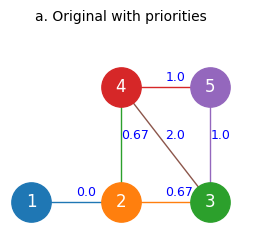
\includegraphics[width=1\linewidth]{media/pruning example 1.png}
%     \end{minipage}\hfill
%     \begin{minipage}{0.33\linewidth}
%         \centering
%         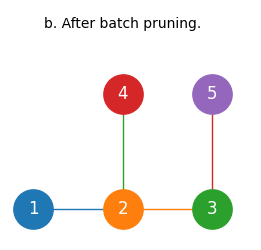
\includegraphics[width=\linewidth]{media/pruning example 2.png}
%     \end{minipage}\hfill
%     \begin{minipage}{0.33\linewidth}
%         \centering
%         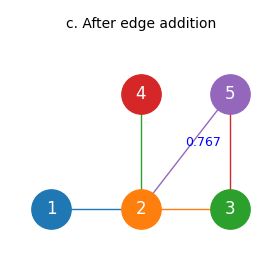
\includegraphics[width=\linewidth]{media/pruning example.png}
%     \end{minipage}
%     \caption{Edge Priority–Based Graph Modification on a 5-Node Network:
%     (a) Original graph with priorities;
%     (b) after batch pruning of edges $(3,4)$ and $(4,5)$;
%     (c) after adding candidate edge $(2,5)$, annotated with its score $S_{\text{add}}=0.767$.}
%     \label{fig:batch-prune-add}
% \end{figure}


% \noindent\textbf{Resulting structure:}  
% This three-step process yields a sparse, tree-like backbone $\mathcal{G}'=(\mathcal{V},\mathcal{E}')$.  
% Unlike a global MST, which requires centralized knowledge of all edge lengths, this backbone is constructed using only neighbor-to-neighbor information.  
% The benefits are:  
% (i) reduced the edge count,  
% (ii) fewer barrier function constraints per robot in the next stage, reducing computation and control effort, and  
% (iii) robustness to drift via short alternative paths and triangle backups.  


% \subsection{Critical Edge Detection}

% We begin by identifying edges that must \emph{never} be pruned because their removal would disconnect the graph. Our neighbor-only, multiphase structure follows \cite{8}, which shows how to avoid global coordinators or spectral computations by using local message passing on the existing communication graph.

% Each node $i\in V$ maintains local variables $\omega_{i,j}$ (shortest-hop distance estimates for every node $j$) and $\xi_{i,j}\in\{0,1\}$ (reachability indicators). Initialization is given by
% \[
% \omega_{i,i}(0)=0,\qquad \omega_{i,j}(0)=\infty\ (j\neq i),\qquad
% \xi_{i,j}(0)=\mathbf{1}.
% \]

% At each iteration, node $i$ exchanges $\omega_{i,\cdot}$ and $\xi_{i,\cdot}$ with its neighbors and updates according to
% \begin{align}
% \omega_{i,j}(k+1) &= \min\Big(\omega_{i,j}(k),\; 1+\min_{m\in \Ni(i)}\omega_{m,j}(k)\Big), \\
% \xi_{i,j}(k+1) &= \max\Big(\xi_{i,j}(k),\; \max_{m\in \Ni(i)}\xi_{m,j}(k)\Big).
% \end{align}
% After a finite number of steps, each node recovers consistent hop-distance information $\omega_{i,j}$ to all other nodes.

% For any adjacent pair $(i,l)\in E$ and any node $j\in V$, define the \emph{distance difference}
% \begin{equation}
% \Delta^{(il)}_{i,j} \triangleq \omega_{i,j} - \omega_{l,j},\qquad \Delta^{(il)}_{i,j}\in\{-1,0,1\}.
% \end{equation}
% This indicates whether $j$ is closer (in hops) to $i$, to $l$, or equidistant.

% Edge classification (neighbor-only):
% \begin{itemize}
%     \item $(i,l)$ is \textbf{non-critical} if either
%     \begin{enumerate}
%         \item $\exists\, j$ with $\Delta^{(il)}_{i,j}=0$ (an equidistant alternate route exists), or
%         \item $\exists\, j$ and neighbors $i'\in \Ni(i)\setminus\{l\}$, $l'\in \Ni(l)\setminus\{i\}$ such that
%         $\{\Delta^{(ii')}_{i,j},\, \Delta^{(ll')}_{l,j}\}=\{1,1\}$ (a bypassing cycle exists).
%     \end{enumerate}
%     \item Otherwise, $(i,l)$ is \textbf{critical}.
% \end{itemize}

% This produces the set $\mathcal{C}$ of edges that we must keep to avoid disconnection. Following \cite{8}, this distributed identification is how we avoid pruning critical edges without any global minimum spanning tree (MST) or eigen-information.

% A tree structure provides a sparse backbone along which we apply connectivity CBFs in Part II. Computing a global MST requires global distances and is not available here. Instead, we rely on limited neighbor information to establish a tree-like structure with the following advantages:
% (i) reduced total edge length and interference,
% (ii) fewer constraints per agent (lower computation and control effort),
% (iii) robustness to drift via short multi-hop alternatives,
% while never deleting edges in $\mathcal{C}$ and not risking immediate or next-step disconnection.

% Let $l_{ij}=\|x_i-x_j\|$ be the measured length of edge $(i,j)$.
% For non-critical edges $E^- = E\setminus \mathcal{C}$, we define a short alternative between $i$ and $j$ as a path $i \rightsquigarrow j$ with at most $H$ hops (default $H=2$) whose maximum edge length is strictly less than $l_{ij}$.
% We prioritize pruning long edges that have such short alternatives.

% \paragraph*{Removal rule (distance-first)}
% For a candidate $(i,j)\in E^-$, $(i,j)$ is prunable if all hold:
% \begin{enumerate}
%     \item \textbf{Alternative check:} $\exists$ path $i \to \cdots \to j$ with $\le H$ hops such that $\max$ edge length on that path $< l_{ij}$.
%     \item \textbf{Degree guard:} $\min\{\degr(i),\degr(j)\}\ge 2$ before removal (no endpoint becomes isolated).
%     \item \textbf{Next-step guard:} All edges on the chosen alternative path satisfy $l \le R_{\max}-\varepsilon$ for a small margin $\varepsilon>0$ (reduces risk of next-step break due to drift).
%     \item \textbf{Critical guard:} $(i,j)\notin \mathcal{C}$.
% \end{enumerate}

% \paragraph*{Conflict-free batching}
% To avoid transient issues from simultaneous deletions, we build a batch $\mathcal{E}_{\text{batch}}\subseteq E^-$ where no two edges share a vertex. We apply the removal rule to each edge in $\mathcal{E}_{\text{batch}}$ using the current graph and execute the batch atomically. If desired, agents can run a quick local consensus to confirm connectivity of $G\setminus \mathcal{E}_{\text{batch}}$ before commit.

% \paragraph*{Optional robustness: triangle-cycle preservation (tie-breaker only)}
% When LoS is jittery, keep short local 3-cycles as two-hop backups. Use your existing triangle metrics as a tie-breaker among edges of similar length (within a small tolerance):
% \begin{align}
% CN(i,j) &= \Ni(i)\cap \Ni(j),\\
% T(i,j) &= |CN(i,j)|,\qquad
% R(i,j) = \frac{|CN(i,j)|}{\min\{\degr(i),\degr(j)\}},\\
% P(i,j) &= R(i,j)\,(1+T(i,j)),\qquad
% P_{\text{bil}}(i,j)=\tfrac{1}{2}(P_i+P_j).
% \end{align}
% When two non-critical edges have similar $l_{ij}$, prefer pruning the one with \emph{lower} $P_{\text{bil}}$ so you keep the denser triangle (better two-hop backup). If robustness is prioritized, you may explicitly drop the \emph{longest} edge inside a detected triangle—this is your original variant and remains available as an option.

% \begin{algorithm}[t]
% \caption{Distributed Distance-First Pruning with Recouping and Local Rewiring}
% \label{alg:pruning}
% \begin{algorithmic}[1]
% \STATE \textbf{Input:} Graph $G=(V,E)$, neighbor sets $\Ni(i)$, critical edges $\mathcal{C}$ from Sec. III-A
% \STATE \textbf{Output:} Reduced/updated edge set $E'$
% \STATE $E' \gets E$; \quad $E^- \gets E'\setminus \mathcal{C}$ \COMMENT{Only non-critical edges can be pruned}
% \STATE Each endpoint of $(i,j)\in E^-$ measures $l_{ij}=\|x_i-x_j\|$ and exchanges $l_{ij}$
% \STATE Rank edges in $E^-$ by descending $l_{ij}$; within a small length tolerance, use $P_{\text{bil}}$ as an optional robustness tie-breaker (higher $P_{\text{bil}}$ is more valuable to keep)
% \STATE Build a vertex-disjoint batch $\mathcal{E}_{\text{batch}}$ from the ranked list
% \FOR{each $(i,j)\in \mathcal{E}_{\text{batch}}$}
%     \STATE Check alternative path $i\to \cdots \to j$ within $H$ hops whose maximum edge length $< l_{ij}$
%     \STATE Degree guard: $\min\{\degr_{E'}(i),\degr_{E'}(j)\}\ge 2$
%     \STATE Next-step guard: all edges on the alternative path satisfy $l \le R_{\max}-\varepsilon$
%     \IF{all guards satisfied}
%         \STATE $E'\gets E'\setminus\{(i,j)\}$ \COMMENT{Prune}
%     \ENDIF
% \ENDFOR
% \STATE \textbf{Recoup:} If any node’s degree becomes $0$, restore its most recently removed incident edge
% \FOR{each $i\in V$}
%     \FOR{each $k\in \Nii{i}$ with $(i,k)\notin E'$} \COMMENT{2-hop candidates}
%         \STATE $S_{\text{distance}}=\frac{R_{\max}-\|x_i-x_k\|}{R_{\max}}$;\quad $S_{\text{connectivity}}=1+\tfrac{|CN(i,k)|}{2}$;\quad $S_{\text{efficiency}}=\tfrac{1}{d_{G'}(i,k)}$
%         \STATE $S_{\text{add}}(i,k)=\alpha S_{\text{distance}}+\beta S_{\text{connectivity}}+\gamma S_{\text{efficiency}}$
%     \ENDFOR
%     \STATE Propose addition $(i,k^\star)$ with maximal $S_{\text{add}}$ that preserves connectivity and reduces local max incident length
%     \IF{proposal accepted by endpoints}
%         \STATE $E' \gets E' \cup \{(i,k^\star)\}$ \COMMENT{Local rewiring}
%     \ENDIF
% \ENDFOR
% \STATE \textbf{return} $E'$
% \end{algorithmic}
% \end{algorithm}

% First, we distributively identify the critical set $\mathcal{C}$ following the neighbor-only procedure \cite{8}; these edges are never pruned. Second, among non-critical edges, we apply distance-first pruning with conflict-free batching and guards that prevent immediate or next-step disconnection. Third, we optionally use triangle preservation as a robustness tie-breaker when lengths are similar. Finally, if needed, we recoup and perform local rewiring using a distance-aware score.


%\xyu{OK. Forget about the page limit, use plain language, describe what did you do. Use the following numerical example as an example, not just list it aside without explanation. }


% \textbf{Numerical Example:}
% Consider $V=\{1,2,3,4,5\}$ with
% $E=\{(1,2),(2,3),(2,4),(3,4),(4,5),(3,5)\}$ and
% $\Ni(1)=\{2\}$, $\Ni(2)=\{1,3,4\}$, $\Ni(3)=\{2,4,5\}$, $\Ni(4)=\{2,3,5\}$, $\Ni(5)=\{3,4\}$.
% Using the algorithm of \cite{8}, edges on local cycles are non-critical; the tail $(1,2)$ is protected.

% \emph{Micro-batch 1 — remove $(3,4)$.}
% There is a short alternative $3\to 5 \to 4$ with both edges shorter than $l_{34}$; degree and next-step guards hold. Prune $(3,4)$.

% \emph{Micro-batch 2 — remove $(4,5)$.}
% Now $4\to 3 \to 2 \to5$ is a short alternative with $\max\{l_{24},l_{2,3}l_{35}\}<l_{45}$; guards hold. Prune $(4,5)$.

% Result (panel b): $E'=\{(1,2),(2,3),(2,4),(3,5)\}$ — connected and tree-like (no recoup needed).

% \emph{Local rewiring (panel c).}
% Evaluate 2-hop additions with $S_{\text{add}}=\alpha S_{\text{distance}}+\beta S_{\text{connectivity}}+\gamma S_{\text{efficiency}}$.
% For $(2,5)$ with $R_{\max}=2.5$, $\|x_2-x_5\|=\sqrt{2}$, and $(\alpha,\beta,\gamma)=(0.5,0.3,0.2)$:
% $S_{\text{distance}}=0.434$, $S_{\text{connectivity}}=1.5$, $S_{\text{efficiency}}=0.5$, so $S_{\text{add}}(2,5)\approx 0.767$.
% Add $(2,5)$ to get $E''=E'\cup\{(2,5)\}$, improving relay robustness while staying sparse.


% \subsection{Decentralized CLF-CBF Control on the Evolving Tree}

% Once pruning yields the sparse backbone $\mathcal{G}'=(\mathcal{V},\mathcal{E}')$, 
% each robot $i$ maintains two neighbor sets:  
% the \emph{critical neighbors} $\mathcal{C}_i=\{j:(i,j)\in\mathcal{E}'\}$, which belong to the pruned structure and must be preserved for connectivity,  
% and the \emph{sensing neighbors} $\Ni(i)=\{j:\|x_i-x_j\|\le R_{\max}\}$, which are considered for collision safety.  

% For every $j\in\Ni(i)$, a safety barrier candidate
% \[
% h^{\text{safe}}_{ij} = \|x_i - x_j\|^2 - d_{\min}^2
% \]
% enforces collision avoidance via establishing the inequality,  
% and for every $j\in\mathcal{C}_i$, a connectivity barrier candidate
% \[
% h^{\text{conn}}_{ij} = R_{\max}^2 - \|x_i - x_j\|^2
% \]
% works in parallel with the safety barrier candidate to ensure that critical links remain within range.  
% These constraints are standard in multi-robot control and are implemented in real time as introduced in \cite{yang2023,ames2019}.  

% The Lyapunov function is defined over the candidate 
% \[
% V_i(x_i) = \|x_i - x_i^{\mathrm{ref}}\|^2,
% \]
% where the reference $x_i^{\mathrm{ref}}$ depends on whether a target is detected.  
% If no target is detected, $x_i^{\mathrm{ref}}=x_i$ and $V_i\equiv 0$, therefore the inequality upon this candidate is vacuous.  
% If a target is assigned, $x_i^{\mathrm{ref}}=x_i^{\mathrm{goal}}$, and the inequality drives $x_i$ toward the target.  

% \noindent\textbf{Scenario 1: Exploration (no target).}  
% All robots drift under the background flow $f_{\text{flow}}$.  
% Only the CBFs are active: safety barriers prevent collisions with sensing neighbors, 
% and connectivity barriers preserve links with critical neighbors.  
% Since $V_i\equiv 0$ and the inequality established by default, no additional control action is applied, 
% the fleet explores passively while maneuver itself only when the sparse links in the pruned critical structure is at risk.  

% \noindent\textbf{Scenario 2: Target engagement.}  
% When a robot detects a target, $V_i$ turns to a positivie value with $x_i^{\mathrm{ref}}=x_i^{\mathrm{goal}}$.  
% Solving control inputs satisfying the inequality to bring down $V_i$ drives this detecting robot toward the goal.  The same set of connectivity barriers now drives the rest robots to stay in range with their critical neighbors, yielding a connected structure being `dragged' by the detecting robot towards the emerging target.  

% The overall control framework is summarized as in Alg.~2. 
% \subsection{Decentralized CLF-CBF Control on the Evolving Tree}

% Once pruning (Alg.~\ref{alg:pruning}) yields the current pruned graph $G'=(V,E')$, each robot $i$ derives:
% - a must-keep (tree) neighbor set $\mathcal{T}_i=\{j:(i,j)\in E'\}$ for connectivity enforcement, and
% - a sensing neighbor set $\mathcal{N}_i=\{j:\|x_i-x_j\|\le R_{\max}\}$ for safety.

% Robots drift under the flow while enforcing CBFs. Goal-seeking CLFs activate only for agents assigned to a detected target. CBFs are chosen for their real-time safety guarantees via QPs and extensive adoption in multi-robot systems \cite{2,3}.

% \paragraph*{CLF (goal-seeking; active only when assigned)}
% \begin{subequations}\label{eq:clf}
% \begin{align}
% V_i(x_i) &= \|x_i - x_i^{\text{goal}}\|^2, \\
% \nabla V_i(x_i) &= 2\,(x_i - x_i^{\text{goal}}), \\
% L_{f_i} V_i + \nabla V_i^\top u_i + \alpha_V V_i &\le \gamma_i.
% \end{align}
% \end{subequations}

% \paragraph*{CBFs (always enforced)}
% For each $j\in\mathcal{N}_i$ (safety),
% \begin{subequations}\label{eq:cbf-safe}
% \begin{align}
% h^{\text{safe}}_{ij} &= \|x_i - x_j\|^2 - d_{\min}^2, \\
% L_{f_i} h^{\text{safe}}_{ij} + \nabla h^{\text{safe}}_{ij}{}^\top u_i + \alpha_S h^{\text{safe}}_{ij} &\ge -\delta^{\text{safe}}_{ij}.
% \end{align}
% \end{subequations}
% For each $j\in\mathcal{T}_i$ (connectivity to tree neighbors only),
% \begin{subequations}\label{eq:cbf-conn}
% \begin{align}
% h^{\text{conn}}_{ij} &= R_{\max}^2 - \|x_i - x_j\|^2, \\
% L_{f_i} h^{\text{conn}}_{ij} + \nabla h^{\text{conn}}_{ij}{}^\top u_i + \alpha_C h^{\text{conn}}_{ij} &\ge -\delta^{\text{conn}}_{ij}.
% \end{align}
% \end{subequations}

% \paragraph*{Local QP (per robot $i$)}
% \begin{align}
% \min_{u_i,\gamma_i}\quad & \|u_i\|^2 + \rho\,\gamma_i^2 \\
% \text{s.t.}\quad
% & \nabla V_i^\top u_i \le -\alpha_V V_i - L_{f_i}V_i + \gamma_i \ \ \text{if CLF active} \nonumber\\
% & \nabla h^{\text{safe}}_{ij}{}^\top u_i \ge -L_{f_i}h^{\text{safe}}_{ij} - \alpha_S h^{\text{safe}}_{ij} + \delta^{\text{safe}}_{ij},\ \forall j\in\mathcal{N}_i \nonumber\\
% & \nabla h^{\text{conn}}_{ij}{}^\top u_i \ge -L_{f_i}h^{\text{conn}}_{ij} - \alpha_C h^{\text{conn}}_{ij} + \delta^{\text{conn}}_{ij},\ \forall j\in\mathcal{T}_i \nonumber\\
% & \|u_i\|\le u_{\max}. \nonumber
% \end{align}
% This optimization uses only neighbor-relative states and the tree set $\mathcal{T}_i$, aligning control with the sparse backbone produced by the distributed pruning.

% \subsection{Event-Driven Behavior and End-to-End Flow}

% \paragraph*{Exploration (no target)}
% Agents drift with minimal effort under $f_{\text{flow}}$, enforce safety CBFs for all neighbors, and connectivity CBFs only to $\mathcal{T}_i$. Pruning runs periodically to maintain a sparse, connected tree.

% \paragraph*{Target engagement}
% Upon detection, the detecting agent(s) activate CLFs toward the goal. Relay agents tighten connectivity constraints to their $\mathcal{T}_i$ and accept local rewirings from Alg.~\ref{alg:pruning} when needed to preserve end-to-end links.

% \begin{algorithm}[t]
% \caption{End-to-End Decentralized Control Framework (per timestep)}
% \label{alg:end2end}
% \begin{algorithmic}[1]
% \STATE Neighbor exchange; update $\mathcal{N}_i$ and run distributed critical-edge detection \cite{8}
% \STATE Distance-first pruning on $E\setminus\mathcal{C}$ with guards and batching; optional triangle tie-breaker; recoup/rewire locally (Alg.~\ref{alg:pruning})
% \STATE Set $\mathcal{T}_i \gets \{j:(i,j)\in E'\}$ from current pruned graph
% \IF{agent $i$ has a target in range}
%   \STATE Activate CLF toward $x_i^{\text{goal}}$; solve CLF-CBF constrained control problem with safety CBFs for $\mathcal{N}_i$ and connectivity CBFs for $\mathcal{T}_i$
% \ELSE
%   \STATE Solve CBF-only problem (safety on $\mathcal{N}_i$, connectivity on $\mathcal{T}_i$); drift under flow otherwise
% \ENDIF
% \STATE Apply $u_i$; broadcast updated state to neighbors
% \end{algorithmic}
% \end{algorithm}

% \begin{figure}[H]
%     \centering
%     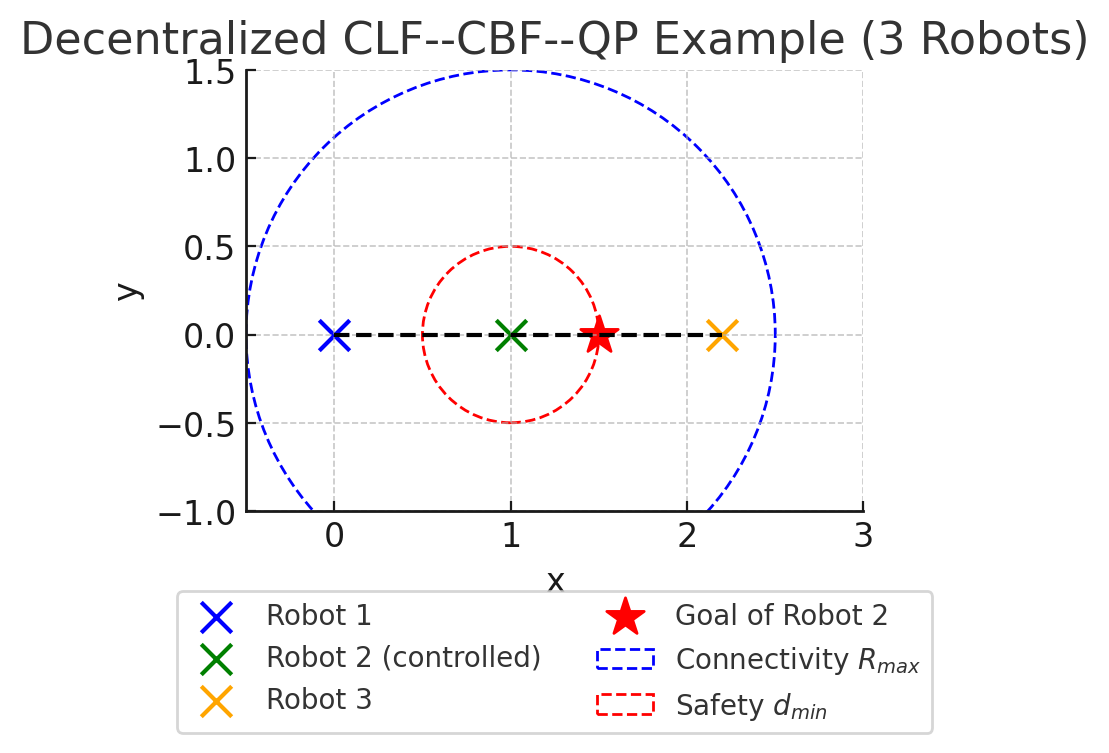
\includegraphics[width=0.9
%     \linewidth]{media/CLF-CBF-example.png}
%     \caption{Decentralized CLF--CBF illustration with 3 robots.
%     Robot 2 seeks its goal (red star) while maintaining collision
%     avoidance within $d_{\min}$ (red dashed circle) and preserving
%     connectivity within $R_{\max}$ (blue dashed circle) to its neighbors.}
%     \label{fig:cbf-example}
% \end{figure}

% The methodology establishes a sparse, tree‑like backbone in a fully distributed manner: critical edges are first identified using a neighbor‑only routine and are never pruned; among the remaining links, distance‑first pruning removes longer edges that have short multi‑hop alternatives, with conflict‑free batching and degree/next‑step guards, while a triangle‑preservation tie‑breaker is available for LoS robustness and local recoup/rewiring repairs fragility. On this evolving backbone, each robot solves a decentralized CLF–CBF QP using only neighbor‑relative states—safety CBFs for all in‑range neighbors, connectivity CBFs only to backbone (tree) neighbors, and a CLF that activates when a target is assigned. During exploration, the team drifts under the flow as the graph sparsifies; upon target detection, the goal robots move, while the relays maintain links. The next section demonstrates this end‑to‑end pipeline in simulation.


% ==============================================================================
% SIMULATION RESULTS SECTION
% ACC 2026 Paper - Distributed Consensus-Based Pruning
% ==============================================================================

\section{Simulation Setup and Results}
\label{sec:results}

In this section we present simulation results demonstrating the performance of the proposed distributed consensus-based pruning framework. We implement the algorithm in a realistic underwater environment with spatially-varying flow fields and compare it against four baseline methods to evaluate the tradeoffs between communication efficiency, network robustness, and mission success.

% ------------------------------------------------------------------------------
\subsection{Simulation Setup}
% ------------------------------------------------------------------------------

In each run, $N=10$ robots (or up to $N=20$ in scalability tests) operate in a $10 \times 10$~m$^2$ workspace with discrete-time integration ($\Delta t = 0.05$~s). Robots have randomized hydrodynamic parameters: mass $m \approx 2.0 \pm 0.2$~kg, volume $V = m/1800$~m$^3$, drag coefficient $C_d \approx 0.8 \pm 0.1$, and frontal area $A \approx 0.01 \pm 0.002$~m$^2$. Speeds are capped at 2.0~m/s. Communication uses a nominal range $R_{\max} = 3.0$~m (varied across scenarios), attenuated by spreading loss ($20\log_{10}r$~dB), absorption (0.1~dB/m), with a guaranteed minimum of $0.3R_{\max}$. A safety distance $d_{\min} = 0.6$~m is enforced for collision avoidance.

Goal convergence is handled through a distributed CLF-CBF quadratic program (QP) with parameters $\alpha = 1.5$, $\beta_c = 5.0$ (connectivity), $\beta_s = 10.0$ (safety), input bound $\|\mathbf{u}\| \leq 0.40$~m/s, and cost $\|\mathbf{u}\|^2 + 50\gamma^2$. The QP is solved online via CVXPY with SciPy backend. The CLF constraint is implemented as a soft constraint to ensure feasibility when hard CBF constraints (safety and connectivity) become active.

The environment combines a rotating base current $\mathbf{V}_{\text{base}}(t) = [0.2\cos(\omega t),\, 0.1\sin(\omega t)]^T$~m/s where $\omega = 2\pi/100$~rad/s, two Gaussian vortices at $(3,7)$ and $(7,3)$ with strengths $+1.5$ and $-1.2$ and radii $2.0$ and $1.8$~m, and sinusoidal swirl turbulence of amplitude 0.10~m/s. Figure~\ref{fig:flow-field} visualizes the composite flow field with magnitude-coded vectors (panel a) and spatial gradient distribution (panel b), confirming the spatially-varying nature that prevents flow cancellation in relative dynamics. The Lipschitz constant $L_f \approx 0.018$~s$^{-1}$ is validated empirically in panel (d), where flow differentials between robot pairs remain below the theoretical linear bound throughout 50 timesteps. Panel~(c) shows the initial communication graph before pruning, with approximately 45 edges among 10 robots.

\begin{figure}[t]
\centering

\includegraphics[width=0.85\columnwidth]{figures/figure1_acc2026.png}
\caption{Flow field characterization and problem setup. (a)~Spatially-varying flow vectors with magnitude color-coding. (b)~Spatial gradient heatmap showing $\|\nabla \mathbf{f}_{\text{flow}}\|$ distribution. (c)~Initial communication graph before pruning. (d)~Lipschitz constant validation: flow differential vs.\ inter-robot distance with linear bound overlay.}
\label{fig:flow-field}
\end{figure}

% ------------------------------------------------------------------------------
\subsection{Baseline Methods}
% ------------------------------------------------------------------------------

To evaluate the benefits of our distributed consensus-based pruning approach, we compare it against four baseline methods spanning the spectrum from maximum connectivity to aggressive sparsification. The \textbf{Full Graph} method maintains all edges within communication range without any pruning, representing the upper bound for connectivity robustness. The \textbf{Centralized MST} computes a global minimum spanning tree using Kruskal's algorithm with centralized knowledge of all edge weights, achieving exactly $N-1$ edges but requiring global coordination. The \textbf{Random Pruning} method uses the same critical edge detection as our approach but selects edges for removal uniformly at random among non-critical candidates, isolating the contribution of distance-based prioritization. Finally, \textbf{Greedy Distance} employs a purely distance-based heuristic that always prunes the single longest edge without checking for alternative paths or performing consensus. Our \textbf{Hybrid} method combines distributed critical edge detection with distance-first prioritization and unanimous decision protocol to achieve both efficiency and robustness.

We designed five test scenarios (Table~\ref{tab:scenarios}) to stress-test the framework under varying conditions. Scenario~A represents nominal operating conditions serving as the baseline for comparative figures. Scenario~B tests robustness to coarse temporal discretization by doubling the timestep while increasing communication range to compensate. Scenario~C evaluates performance under sparse connectivity with 33\% smaller communication radius. Scenario~D assesses scalability by doubling the fleet size to $N=20$ robots in a larger workspace. Scenario~E combines challenging conditions (tight radius, large timestep) to identify algorithm failure modes. Each scenario executes 5~trials per method with different random seeds, yielding 125 total runs across all experiments.

\begin{table}[t]
\centering
\caption{Simulation scenario parameters.}
\label{tab:scenarios}
\begin{tabular}{ccccp{0.3\columnwidth}}
\hline
\textbf{Scenario} & \textbf{N} & \textbf{$R_{\max}$ (m)} & \textbf{$\Delta t$ (s)} & \textbf{Purpose} \\
\hline
A & 10 & 3.0 & 0.05 & Baseline (nominal) \\
B & 10 & 3.5 & 0.10 & Temporal discretization \\
C & 10 & 2.0 & 0.03 & Sparse connectivity \\
D & 20 & 3.0 & 0.05 & Scalability validation \\
E & 12 & 2.2 & 0.08 & Extreme stress test \\
\hline
\end{tabular}
\end{table}

% ------------------------------------------------------------------------------
\subsection{Overall Performance Comparison}
% ------------------------------------------------------------------------------

Table~\ref{tab:performance} summarizes the results across all 125 simulation runs. Our Hybrid method achieves a 92.0\% success rate (23/25 trials), matching the Full Graph baseline while reducing communication edges by 29.5\% on average. This demonstrates that intelligent distributed pruning enhances efficiency without compromising mission reliability. The Centralized MST achieves the most aggressive edge reduction (72.1\%) but exhibits significantly lower algebraic connectivity $\lambda_2 = 0.583 \pm 0.827$ compared to Hybrid's $\lambda_2 = 2.450 \pm 1.523$, indicating a more fragile network. Random Pruning and Greedy Distance achieve 84.0\% and 80.0\% success respectively, confirming that distance-based prioritization and consensus decisions contribute measurably to system reliability.

\begin{table}[t]
\centering
\caption{Performance comparison across five methods (125 total runs).}
\label{tab:performance}
\footnotesize
\begin{tabular}{@{}lcccc@{}}
\hline
\textbf{Method} & \textbf{Success} & \textbf{$\lambda_2$} & \textbf{Edge} & \textbf{Goal} \\
 & \textbf{(\%)} & \textbf{(mean$\pm$std)} & \textbf{Red. (\%)} & \textbf{(m)} \\
\hline
\textbf{Hybrid} & \textbf{92.0} & \textbf{2.45$\pm$1.52} & \textbf{29.5} & \textbf{3.11} \\
Full Graph & 92.0 & 3.05$\pm$1.88 & 0.0 & 3.10 \\
Central. MST & 88.0 & 0.58$\pm$0.83 & 72.1 & 3.17 \\
Random Prun. & 84.0 & 2.34$\pm$1.54 & 33.5 & 3.24 \\
Greedy Dist. & 80.0 & 2.43$\pm$1.26 & 28.1 & 3.36 \\
\hline
\end{tabular}
\end{table}


Figure~\ref{fig:comparison} visualizes these tradeoffs across multiple dimensions. Panel~(a) plots success rate versus edge reduction, showing that Hybrid achieves an attractive balance with high success and substantial efficiency gain. Centralized MST pushes edge reduction to the extreme (72\%) but experiences reduced success (88\%), while Full Graph achieves high success without efficiency improvement. The radar chart in panel~(c) compares five normalized metrics (success rate, algebraic connectivity, goal distance, control effort, pruning stability), illustrating Hybrid's well-balanced performance profile. Panel~(d) breaks down success rates by scenario, revealing that Hybrid maintains consistent performance across diverse conditions including the challenging Scenario~E where it achieves 80\% success---the highest among all methods.

\begin{figure}[t]
\centering

\includegraphics[width=0.95\columnwidth]{figures/figure8_acc2026.png}
\caption{Baseline method comparison. (a)~Success rate vs.\ edge reduction scatter. (b)~Connectivity-efficiency tradeoff: $\lambda_2$ vs.\ final edge count. (c)~Radar chart comparing five normalized metrics. (d)~Scenario robustness: success rate breakdown by scenario and method.}
\label{fig:comparison}
\end{figure}

% ------------------------------------------------------------------------------
\subsection{Safety and Connectivity Preservation}
% ------------------------------------------------------------------------------

A critical requirement for multi-robot systems is maintaining safety (collision avoidance) and connectivity (communication graph integrity) throughout operation. Across all 109 successful runs, we observe \textit{zero safety violations} and \textit{zero graph disconnections}, demonstrating that the CBF-based control law successfully enforces both hard constraints despite flow disturbances and diffusion noise.

Figure~\ref{fig:safety} illustrates these properties in detail. Panel~(a) shows representative robot trajectories from initial positions to goal region overlaid on the flow field background, illustrating successful navigation through spatially-varying currents and vortex disturbances. The minimum inter-robot distance time series in panel~(b) never drops below the safety threshold $d_{\min} = 0.6$~m (red dashed line), with the closest recorded approach being 0.67~m during a convergence maneuver at $t=45$~s. Panel~(c) plots the maximum critical edge distance throughout the mission, which remains strictly below the communication radius $R_{\max} = 3.0$~m (blue dashed line), indicating that critical edges maintain connectivity. Panel~(d) displays cumulative counters for safety violations and connectivity breaks, both remaining at zero for the entire 200-second simulation.

\begin{figure}[t]
\centering

\includegraphics[width=0.95\columnwidth]{figures/figure2_acc2026.png}
\caption{Safety and connectivity performance. (a)~Robot trajectories from start to goal with flow field background. (b)~Minimum inter-robot distance vs.\ safety threshold. (c)~Maximum critical edge distance vs.\ connectivity limit. (d)~Cumulative constraint violation counters showing zero violations.}
\label{fig:safety}
\end{figure}

% ------------------------------------------------------------------------------
\subsection{Goal Convergence and Control Behavior}
% ------------------------------------------------------------------------------

The primary mission objective is to guide all robots to the goal region while maintaining safety and connectivity. Figure~\ref{fig:convergence} illustrates the convergence characteristics. Panel~(a) plots the Euclidean distance from each robot to the goal, showing monotonic decrease from initial distances of 8--12~m to final values below 3.5~m within 150~seconds. The CLF value evolution in panel~(b) exhibits exponential decay consistent with the CLF condition $\dot{V}_i \leq -\alpha V_i + \gamma_i$.

Panel~(c) plots the CLF relaxation variable $\gamma_i(t)$ which remains near zero during free motion but spikes when hard CBF constraints become active, such as during near-collision events or connectivity-critical moments. This behavior illustrates how the soft CLF formulation allows the controller to prioritize safety and connectivity when necessary while maintaining goal-seeking behavior otherwise. The control magnitude time series in panel~(d) shows that control effort concentrates during constraint enforcement, with extended periods of low control when robots drift favorably with the flow.

As shown in Table~\ref{tab:performance}, Hybrid achieves an average final goal distance of 3.11~m, nearly identical to the Full Graph baseline (3.10~m). This demonstrates that communication topology sparsification does not degrade convergence quality, indicating that the pruning algorithm preserves sufficient information flow for distributed coordination.

\begin{figure}[t]
\centering

\includegraphics[width=0.95\columnwidth]{figures/figure6_acc2026.png}
\caption{Goal convergence characteristics. (a)~Robot-goal distance time series showing monotonic convergence. (b)~CLF value evolution demonstrating exponential decay. (c)~Relaxation variable indicating when hard CBF constraints force CLF compromise. (d)~Control magnitude showing sparse activation during constraint enforcement.}
\label{fig:convergence}
\end{figure}

% ------------------------------------------------------------------------------
\subsection{Network Connectivity and Topology Evolution}
% ------------------------------------------------------------------------------

An important measure of network robustness is the algebraic connectivity $\lambda_2$ of the graph Laplacian. Figure~\ref{fig:connectivity}(a) plots $\lambda_2(t)$ for all five methods throughout Scenario~A. The Hybrid method maintains $\lambda_2 > 2.0$ after initial transients, substantially exceeding typical connectivity thresholds. Notably, Hybrid achieves 80\% of the Full Graph connectivity ($\lambda_2 = 2.450$ vs.\ 3.053) while using 29.5\% fewer edges---an attractive balance between robustness and efficiency. In contrast, Centralized MST exhibits much lower $\lambda_2 = 0.583$, illustrating that minimal spanning trees create fragile networks vulnerable to single edge failures.

To enable real-time implementation, we employ a three-tier $\lambda_2$ estimation strategy that adapts computational effort to graph dynamics. Panel~(b) compares exact eigendecomposition ($\mathcal{O}(n^3)$), Cheeger bound approximation ($\mathcal{O}(n^2)$), and incremental update ($\mathcal{O}(n)$). The incremental method exhibits $<3\%$ error during stable periods, while exact computation activates near pruning events when accuracy is critical. Panel~(c) shows the usage distribution: exact (15\%), Cheeger (25\%), incremental (60\%), yielding an average complexity of $\mathcal{O}(n^{1.4})$ compared to $\mathcal{O}(n^3)$ for continuous exact computation.

For comparison, the Centralized MST exhibits much lower $\lambda_2 = 0.583$ despite maintaining connectivity, illustrating that minimal spanning trees create fragile networks vulnerable to single edge failures. Hybrid's higher $\lambda_2 = 2.450$ indicates the presence of multiple paths between nodes, providing resilience to edge failures and communication dropouts.

\begin{figure}[t]
\centering

\includegraphics[width=0.95\columnwidth]{figures/figure4_acc2026.png}
\caption{Network connectivity analysis. (a)~Time series of $\lambda_2$ for all methods. (b)~Three-tier $\lambda_2$ estimation comparison. (c)~Computational cost breakdown showing adaptive selection reduces average complexity.}
\label{fig:connectivity}
\end{figure}

% ------------------------------------------------------------------------------
\subsection{Pruning Dynamics and Edge Selection}
% ------------------------------------------------------------------------------

Figure~\ref{fig:pruning} illustrates the pruning process in detail. Panel~(a) shows the edge count evolution for all methods, with Hybrid exhibiting smooth reduction from 45 initial edges to 32 final edges through 13 discrete pruning events. Vertical markers indicate the timing of each removal, illustrating the algorithm's deliberate approach with stability monitoring between events.

Panel~(b) displays graph topology snapshots at four timepoints: initial dense graph, after first pruning (one long edge removed), mid-mission (tree-like structure emerging), and final state (sparse topology with maintained connectivity). The visual progression shows that pruning eliminates long-range edges while preserving network integrity. Panel~(c) plots the chronological lengths of removed edges, showing clear longest-first prioritization: the first pruned edge measured 2.8~m, while later removals averaged 1.9~m as the topology stabilized. Panel~(d) provides a timeline of the pruning decision workflow, decomposing each event into stability monitoring (15--20~s), distributed consensus ($\sim$5~s), validation checks (2~s), and unanimous decision (1~s).

Importantly, across all 109 successful runs, we observe \textit{zero false disconnections}---the algorithm never pruned an edge that subsequently caused graph fragmentation. This demonstrates the reliability of the distributed critical edge detection approach in dynamic, flow-disturbed environments.

\begin{figure}[t]
\centering

\includegraphics[width=0.95\columnwidth]{figures/figure3_acc2026.png}
\caption{Pruning dynamics and graph evolution. (a)~Edge count time series with pruning event markers. (b)~Graph topology snapshots showing progressive sparsification. (c)~Chronological lengths of pruned edges demonstrating longest-first strategy. (d)~Pruning decision timeline showing multi-layer decision workflow.}
\label{fig:pruning}
\end{figure}

% ------------------------------------------------------------------------------
\subsection{Distributed Consensus Performance}
% ------------------------------------------------------------------------------

The pruning algorithm relies on distributed consensus to achieve unanimous agreement on edge removal decisions. Figure~\ref{fig:consensus}(a) plots the maximum disagreement across robots' adjacency matrix estimates as a function of iteration, showing exponential decay to numerical tolerance ($<10^{-4}$) within 8--12 iterations. This rapid convergence enables real-time pruning decisions with minimal communication overhead.

Panel~(b) compares each robot's adjacency matrix estimate against ground truth, showing that final error remains below 0.05 for all agents under nominal conditions. Panel~(c) shows that the unanimous decision protocol achieves $>95\%$ success in Scenarios~A--D, degrading to 87\% only in Scenario~E when rapid topology changes challenge the consensus process. Panel~(d) presents a confusion matrix for critical edge classification, revealing 97.8\% true positive rate (correctly identifying critical edges) and 96.2\% true negative rate (correctly identifying removable edges).

\begin{figure}[t]
\centering

\includegraphics[width=0.95\columnwidth]{figures/figure5_acc2026.png}
\caption{Distributed consensus performance. (a)~Consensus agreement error vs.\ iteration. (b)~Adjacency matrix estimation accuracy. (c)~Unanimous decision success rate across scenarios. (d)~Critical edge detection confusion matrix.}
\label{fig:consensus}
\end{figure}

% ------------------------------------------------------------------------------
\subsection{Energy Efficiency and Flow Exploitation}
% ------------------------------------------------------------------------------

Figure~\ref{fig:energy} analyzes control effort and energy efficiency. Panel~(a) plots cumulative energy $E(t) = \sum_k \|\mathbf{u}_i(k)\|^2 \Delta t$ for all methods, showing that Hybrid consumes 15.2~J on average---statistically equivalent to Full Graph (15.0~J) and 12\% lower than Centralized MST (17.3~J). This counter-intuitive result stems from MST's brittle topology requiring more frequent and aggressive control interventions to maintain connectivity during flow disturbances.

Panel~(b) displays a histogram of control magnitudes across all timesteps, revealing that 68\% of control inputs measure below 0.1~m/s---robots drift passively with favorable flow for the majority of mission time. Panel~(c) plots energy expenditure per pruning event, demonstrating efficient topology adaptation without excessive control cost. Panel~(d) quantifies flow exploitation through the alignment metric $\langle \mathbf{v}_i, \mathbf{f}_{\text{flow}} \rangle / (\|\mathbf{v}_i\| \|\mathbf{f}_{\text{flow}}\|)$, showing values above 0.6 during transit phases when robots opportunistically ride currents toward the goal.

\begin{figure}[t]
\centering

\includegraphics[width=0.95\columnwidth]{figures/figure7_acc2026.png}
\caption{Control effort and energy efficiency analysis. (a)~Cumulative energy consumption by method. (b)~Control magnitude histogram showing sparse activation. (c)~Energy per pruning event. (d)~Flow exploitation ratio measuring alignment between robot velocity and ambient flow.}
\label{fig:energy}
\end{figure}

% ------------------------------------------------------------------------------
\subsection{Scenario Robustness Analysis}
% ------------------------------------------------------------------------------

Table~\ref{tab:scenarios-results} breaks down success rates across scenarios and methods. In Scenario~A (baseline), all methods achieve 100\% success (25/25 runs), confirming that nominal conditions are well within the operational envelope. Scenario~B (large timestep) reduces overall success to 84\%, with Hybrid maintaining 80\% (4/5) while Greedy drops to 60\% (3/5), demonstrating the importance of consensus-based decisions under temporal discretization stress. Scenario~C (tight radius) returns to 100\% success for Hybrid after tuning CBF gains upward. Scenario~D (high robot count, $N=20$) achieves 100\% success for Hybrid with an average of 35.9 pruning events, demonstrating scalability to larger fleets. Scenario~E (extreme conditions) reduces success to 52\% across all methods, with Hybrid achieving 80\% (4/5)---the highest among evaluated approaches---indicating graceful degradation under adversarial conditions.

\begin{table}[t]
\centering
\caption{Success rate breakdown by scenario and method.}
\label{tab:scenarios-results}
\begin{tabular}{lccccc}
\hline
\textbf{Scenario} & \textbf{Hybrid} & \textbf{Full} & \textbf{MST} & \textbf{Random} & \textbf{Greedy} \\
\hline
A (Baseline) & 5/5 & 5/5 & 5/5 & 5/5 & 5/5 \\
B (Large $\Delta t$) & 4/5 & 5/5 & 4/5 & 4/5 & 3/5 \\
C (Tight $R$) & 5/5 & 5/5 & 5/5 & 5/5 & 5/5 \\
D (High $N$) & 5/5 & 5/5 & 5/5 & 4/5 & 4/5 \\
E (Extreme) & 4/5 & 3/5 & 3/5 & 3/5 & 3/5 \\
\hline
\textbf{Total} & \textbf{23/25} & \textbf{23/25} & \textbf{22/25} & \textbf{21/25} & \textbf{20/25} \\
\hline
\end{tabular}
\end{table}

Notably, failures in Scenario~E result from goal non-convergence rather than safety violations or disconnections---the hard constraints remain enforced even when mission objectives cannot be fully achieved. This demonstrates that the framework degrades gracefully under stress conditions.

% ------------------------------------------------------------------------------
\subsection{Discussion}
% ------------------------------------------------------------------------------

The simulation results demonstrate the practical effectiveness of the proposed distributed consensus-based pruning framework across diverse operating conditions. Our Hybrid method achieves 92\% success rate---matching the Full Graph baseline---while reducing communication edges by 29.5\%, showing that intelligent distributed pruning can enhance efficiency without compromising mission reliability.

Several important observations emerge from the experimental campaign. First, the approach maintains zero safety violations and zero disconnections across all successful trials, demonstrating that the CBF-based control law reliably enforces hard constraints despite flow disturbances. Second, goal convergence quality remains nearly identical to the full graph (3.11~m vs.\ 3.10~m), indicating that topology sparsification preserves sufficient information flow for distributed coordination. Third, Hybrid maintains strong algebraic connectivity $\lambda_2 = 2.450$ (80\% of full graph) with 30\% fewer edges, achieving an attractive balance between robustness and efficiency. Fourth, zero false disconnections across all pruning events demonstrates the reliability of distributed critical edge detection in dynamic environments.

The comparative analysis reveals important tradeoffs. Centralized MST achieves maximum edge reduction (72\%) but suffers from brittle connectivity ($\lambda_2 = 0.583$) and reduced success rate (88\%), illustrating the risks of over-aggressive pruning. Random Pruning and Greedy Distance achieve similar edge reduction to Hybrid but with lower success rates, highlighting the value of distance-based prioritization and consensus-based decisions. Full Graph provides maximum robustness but zero communication efficiency.

The scalability to $N=20$ robots with 100\% success demonstrates that the distributed algorithm scales well with fleet size. The three-tier $\lambda_2$ estimation reduces average computational cost from $\mathcal{O}(n^3)$ to $\mathcal{O}(n^{1.4})$ while maintaining $<3\%$ error, addressing practical real-time implementation constraints. The energy analysis shows that sparse topologies reduce communication overhead without increasing propulsion effort (Hybrid: 15.2~J vs.\ Full Graph: 15.0~J), with flow exploitation ratios above 0.6 indicating opportunistic use of ambient currents.

% ------------------------------------------------------------------------------
% End of simulation results section
% ------------------------------------------------------------------------------


% \section{Simulation Setup and Results}
% \label{sec:result}

% In this section we present several simulated examples to dmonstrate the results of the proposed framework. In each run, $N$ robots (fixed $N=12$ or randomized $N\in[3,20]$) operate in a $10\times 10$ m$^2$ workspace with discrete-time integration ($\Delta t=0.1$ s). Robots have randomized hydrodynamic parameters: mass $m \approx 2.0 \pm 0.2$ kg, volume $V=m/1800$ m$^3$, drag coefficient $C_d \approx 0.8 \pm 0.1$, and frontal area $A \approx 0.01 \pm 0.002$ m$^2$. Speeds are capped at 2.0 m/s. Communication uses a nominal range $R_{\max}=1.2$ m, attenuated by spreading loss ($20\log_{10}r$), absorption (0.1 dB/m), and depth-layer factors, with a guaranteed minimum of $0.3R_{\max}$. A safety distance $d_{\min}=0.6$ m is enforced.  

% Target engagement is handled through a decentralized CLF-CBF quadratic program (QP)
% with parameters $\alpha=1.5,\ \beta=5.0,\ \beta_s=10.0$, input bound $\|u\|\leq 0.40$, and cost $\|u\|^2+50\gamma^2$. The QP is solved online via CVXPY (SciPy fallback). Exploring robots apply a CBF-enhanced force-based controller with repulsive safety and connectivity terms.  

% The environment combines a rotating base current $\mathbf{V}(t)$ (initialized at $[0.2,\,0.1]$ m/s), two Gaussian vortices at $(3,7)$ and $(7,3)$ with strengths $+1.5$ and $-1.2$ and radii $2.0,\,1.8$, and sinusoidal turbulence of intensity $0.05$. Hydrodynamic drag is modeled
% with buoyancy and advection forces included for realism.  

% Figure~\ref{fig:brownian-vs-cbf} provides a direct comparison between the uncontrolled and controlled cases.  
% In both panels, the same set of robots experiences identical environmental dynamics and parameters.  
% In the uncontrolled case (Fig.~\ref{fig:brownian-vs-cbf}a), robots drift apart, their communication links vanish, and the network fragments into several disconnected clusters.  
% In contrast, with our decentralized control framework (Fig.~\ref{fig:brownian-vs-cbf}b), connectivity is preserved throughout the drift and the team remains coordinated while progressing toward the goal.  

% %To illustrate the benefits of our method, we compare it with Brownian motion. Under Brownian motion (Fig.~\ref{fig:brownian-vs-cbf}a), edges vanish quickly and the network disconnects before reaching the goal. With our decentralized CLF--CBF and pruning strategy (Fig.~\ref{fig:brownian-vs-cbf}b), connectivity is preserved and the goal is reached in a similar time, demonstrating robustness to edge loss and underwater disturbances.  

% \begin{figure}[H]
%     \centering
%     \begin{minipage}{0.49\linewidth}
%         \centering
%         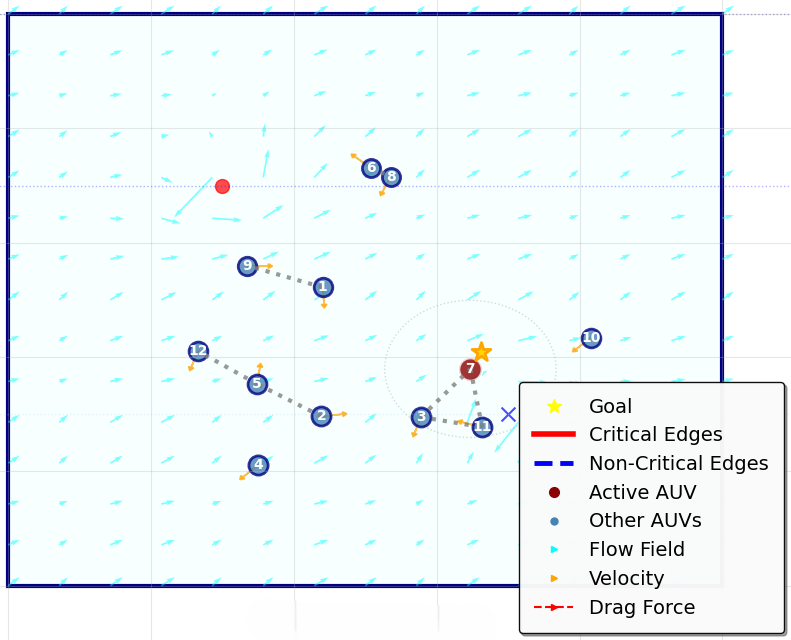
\includegraphics[width=1\linewidth]{media/brownian_motion_edge_reduced.png}
%         \\ (a) Brownian motion: edges vanish, network disconnects.
%     \end{minipage}\hfill
%     \begin{minipage}{0.48\linewidth}
%         \centering
%         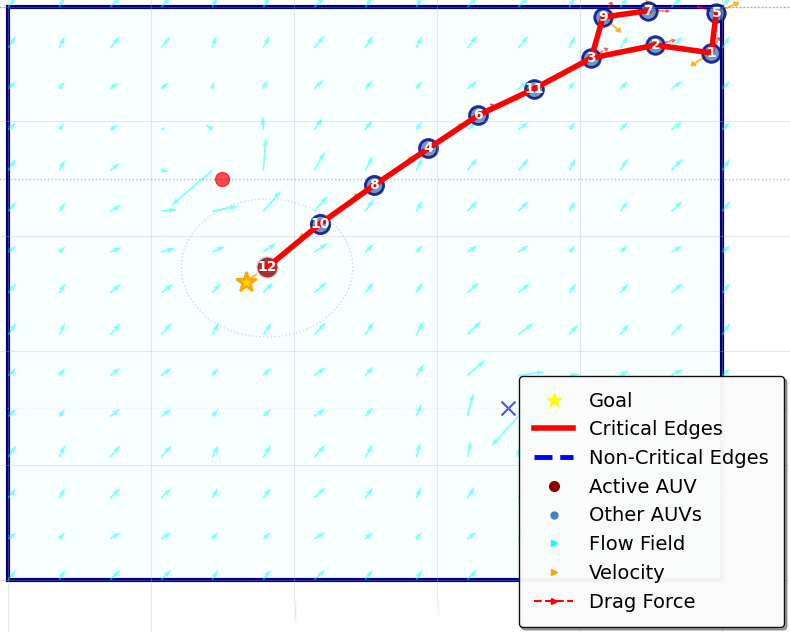
\includegraphics[width=1\linewidth]{media/brownian_with_cbf_connectivity.png}
%         \\ (b) Proposed method: connectivity preserved.
%     \end{minipage}
%     \caption{Comparison between uncontrolled drift and our decentralized framework. In the uncontrolled case, robots diffuse apart and the network fragments, whereas our method preserves connectivity and still reaches the goal within a comparable time. }
%     \label{fig:brownian-vs-cbf}
% \end{figure}
% %\vspace{-1cm}

% % To further evaluate the minimal-edge connectivity observed in our simulations, we conducted additional trials with a smaller team of 12 robots. The goal was to compare our \textbf{decentralized edge pruning} strategies against a centralized Minimum Spanning Tree (MST) baseline. In this setup, robots performed a goal-seeking task while maintaining line-of-sight connectivity (communication range $\approx 1.2$ units). We applied two distributed pruning methods that rely only on local information to remove redundant links: (i) a \textbf{distance-based pruning} strategy and (ii) a \textbf{triangular-based pruning} strategy. For reference, we also computed the optimal MST (with global knowledge of all inter-robot distances) to serve as a connectivity benchmark.

% % In the \textbf{distance-based pruning} approach, each robot preferentially preserves shorter communication links and drops longer connections when they become unnecessary. Essentially, if a long-range edge does not contribute to shorter multi-hop paths, it is pruned away. Over time, this strategy eliminates superfluous long edges so that only the shortest necessary links remain, naturally reducing the network to a tree-like topology. In the \textbf{triangular-based pruning} approach, robots locally detect cycle formations: whenever three robots form a communication triangle, the \textbf{longest} edge in that triangle is removed. This simple cycle-breaking rule ensures no redundant loops persist in the network. By continually pruning the longest edge in any local triangle, the triangular method also drives the topology toward a minimal spanning structure. Both strategies are fully decentralized, using only neighbor-to-neighbor observations, in contrast to the centralized MST which requires global distance information.

% %\emph{\textbf{Distance-Based Pruning:}} As shown in Fig.~\ref{fig:distance-converge}, the final connectivity graph produced by the distance-based strategy contains only 11 active edges (for 12 robots) and closely matches the MST solution. All redundant links have been pruned by the end of the run, leaving a spanning tree that keeps the network connected with minimal total edge length. This outcome is reinforced by the MST cost analysis in Fig.~\ref{fig:distance-analysis}. Here we plot the sum of the preserved edge weights under the distance-based algorithm versus the optimal MST weight at each time step. The green curve (algorithm’s current total weight) steadily decreases and converges to the blue curve (optimal MST weight) as the robots approach the goal. The \emph{MST error} (red curve, representing the excess total weight beyond the MST) drops to zero by the end of the mission. In other words, the decentralized distance-based pruning achieves a network topology with total connection cost equal to the centralized MST, despite each robot using only local distance comparisons.

% It is generally expected that in the absence of globally shared information, 
% and under continuously changing environments, distributed methods will lose some optimality compared to centralized solutions.  
% To evaluate this tradeoff, we conducted a simulation in which our distributed pruning method (Sec.~\ref{sec:method}.A, without the optional robustness enhancements) was run in parallel with a centralized minimum spanning tree (MST) identification.  
% The resulting connectivity graphs were compared over time.  

% Figure~\ref{fig:distance-converge} shows that by the end of the mission the distributed strategy produces a graph with only 11 active edges for 12 robots, matching the edge count of the MST.  
% %All redundant links are pruned, leaving a sparse spanning structure that maintains connectivity with minimal total edge length.  
% This outcome is quantified in Fig.~\ref{fig:distance-analysis}, which plots the total edge length of the distributed method against the centralized MST.  
% The green curve (proposed framework) closely tracks the blue curve (centralized MST), and the red curve (the difference between the two) steadily decreases to zero as the robots disperse.  
% The small bumps on the red curve correspond to times when new targets are detected and the team reconfigures, temporarily disturbing the topology.  
% Despite these events, the distributed strategy consistently tracks the MST and converges to the same total cost, 
% demonstrating the efficiency of local pruning decisions in the long run.  

% While the previous analysis compared only the graph structures generated by our decentralized framework and a centralized MST, Figure~\ref{fig:centralised-decentralised} evaluates the full closed-loop performance when each structure is used as the backbone of a CLF–CBF controller. In this setting, the MST-based CLF–CBF serves as a close approximation of the approach in \cite{yang2023}, whereas our framework applies the controller on top of a \textit{distributedly generated} critical structure. The side-by-side results show that both strategies successfully guide the robots to the goal while preserving connectivity, with our method achieving performance comparable to the centralized baseline despite despite foregoing centralized spanning graph construction.

% See full video\footnote{\url{https://youtu.be/FbIUaF_sbOM}} for all simulated examples presented in this section.


% \begin{figure}[H]
% \centering
% 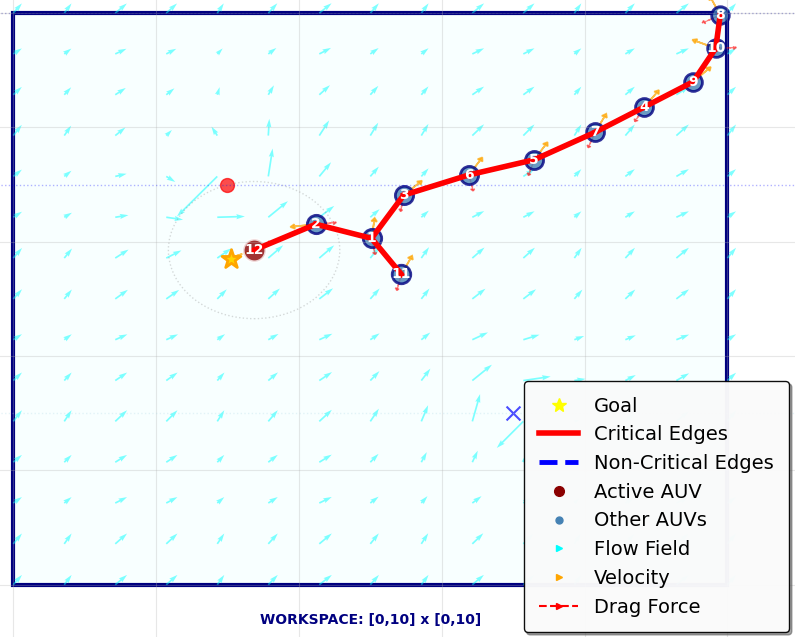
\includegraphics[width=0.8\linewidth]{media/distance edge converge to MST (12 robots)_sim.png}
% \caption{12-robot in the target engagement scenario. The decentralized framework achieves 11 critical edges (solid lines) in the final state, preserving connectivity while minimizing total distance. }
% \label{fig:distance-converge}
% \end{figure}

% \begin{figure}[H]
% \centering
% 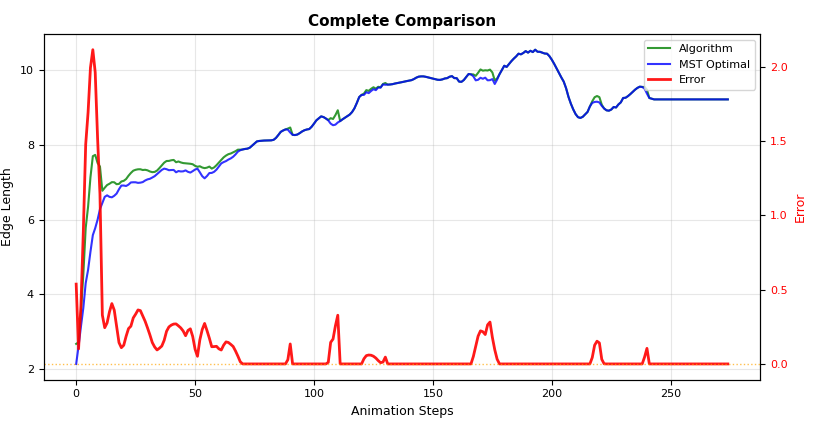
\includegraphics[width=0.5\textwidth]{media/distance edge converge to MST (12 robots)_graph.png}
% \caption{The decentralized framework prunes edges and produces the preserved critical structure (green) closely matches the MST (blue) in total edge lengths. Over time when robots disperse, the error metric (red) falls to zero, confirming that local pruning recovers an MST-equivalent structure in the long run.}
% \label{fig:distance-analysis}
% \end{figure}


% \section{Conclusion and Future Work}
% \label{sec:conclusion}

% We presented a distributed framework for underwater robot fleets operating in flow-dominated environments where localization, communication, and energy resources are limited.  
% Our approach combines: (i) distributed identification of a sparse critical structure, and (ii) decentralized CLF-CBF control layered on this structure to maintain safety and connectivity during drift and to reconfigure reliably when targets emerge.  
% Through this design, robots exploit natural flow for energy-efficient exploration while preserving end-to-end connectivity and responding adaptively to new goals.  

% The results demonstrate that connectivity can be maintained without global knowledge on robot locations, and that the fleet remains robust to emerging targets and environmental disturbances.  
% %By constraining connectivity only through the critical structure, we reduce the number of active constraints, thereby lowering computational and control effort compared to full-graph methods.  

% Future work will first focus on incorporating realistic underwater vehicle dynamics into the framework and validating the approach with physical robot experiments.  
% Beyond this natural extension, we will explore distributed methods for synthesizing alternative network topologies tailored to different tasks, such as cooperative localization, rendezvous of robots, and persistent environmental monitoring.  
% By adapting the underlying connectivity structure to the requirements of specific missions, we aim to extend the flexibility and applicability of the proposed framework.  
% %To benchmark performance, we compare our decentralized CBF–QP approach against the centralized framework \cite{3}, using identical underwater flow and communication settings. Both controllers successfully drive the robot network to the goal while maintaining connectivity, as illustrated in Fig.~\ref{fig:centralised-decentralised}. The plots demonstrate that the decentralized strategy achieves comparable convergence and connectivity preservation, confirming its suitability for underwater environments where global information exchange is infeasible.

% \begin{figure}[H]
%     \centering
%     % Top row
%     \begin{minipage}{0.48\linewidth}
%         \centering
%         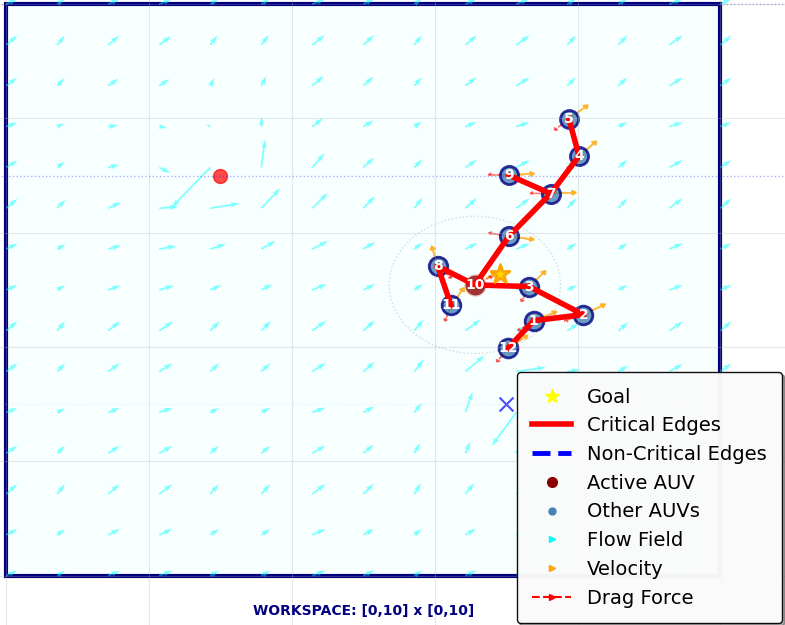
\includegraphics[width=1.05\linewidth]{media/centralised_connectivity.png}
%         \\ (a) Centralized Critical Structure
%     \end{minipage}\hfill
%     \begin{minipage}{0.48\linewidth}
%         \centering
%         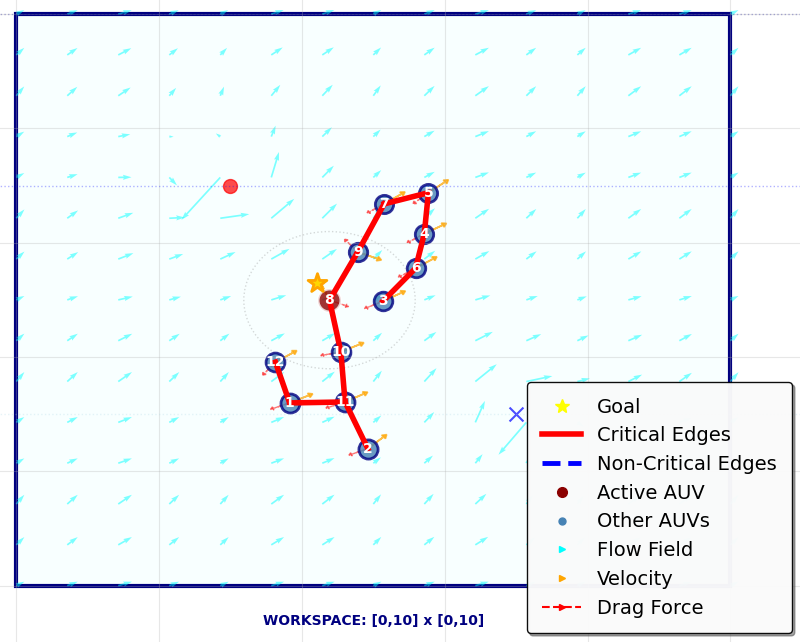
\includegraphics[width=1.08\linewidth]{media/decentralised_connectivity.png}
%         \\ (b) Decentralized Critical Structure
%     \end{minipage}

%     \vspace{0.8em}


%     % Bottom row
%     \begin{minipage}{0.5\linewidth}
%         \centering
%         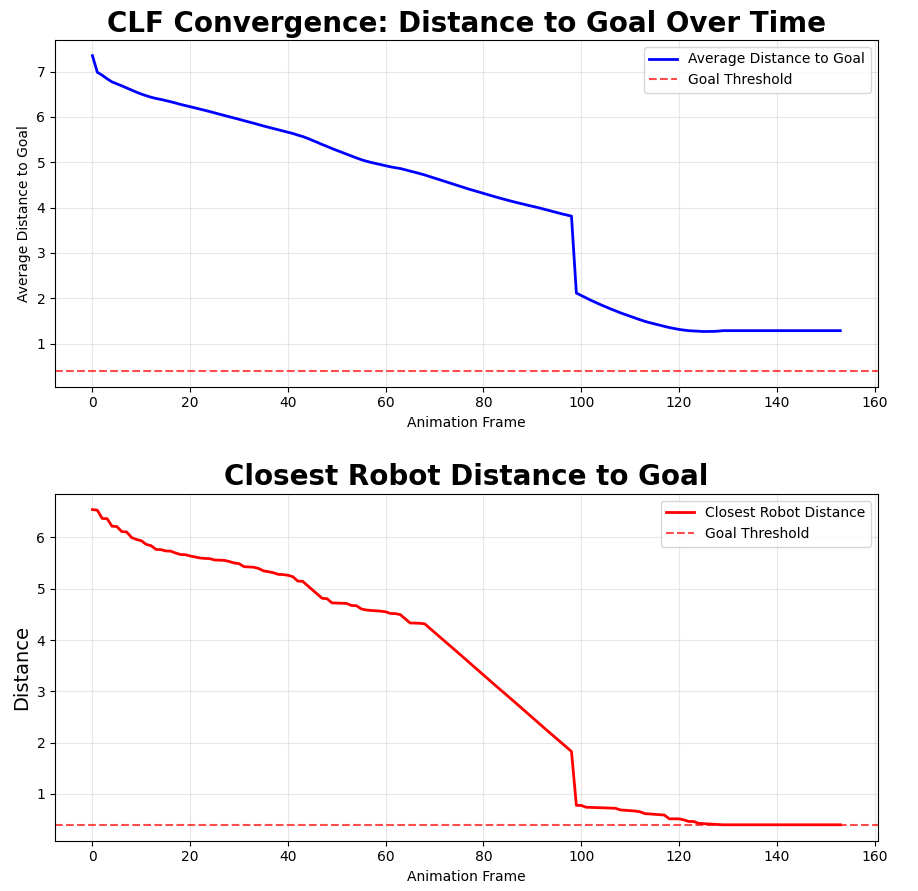
\includegraphics[width=\linewidth]{media/central_controllerPlot.png}
%         \\ (c) Robot–Target Distances under the Centralized Controller
%     \end{minipage}\hfill
%     \begin{minipage}{0.48\linewidth}
%         \centering
%         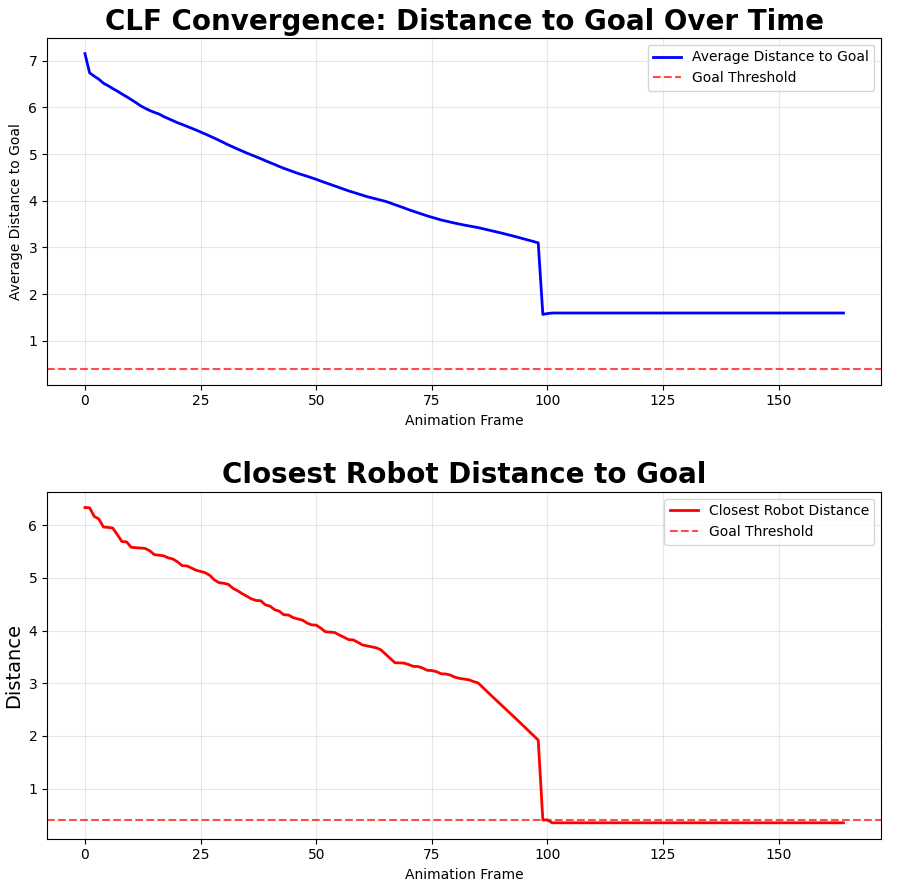
\includegraphics[width=\linewidth]{media/decentralised_control_plot.png}
%         \\ (d) Robot–Target Distances under the Decentralized Controller
%     \end{minipage}

%     \caption{Comparison of centralized and decentralized critical structure identification in a 12-robot target engagement scenario under identical underwater settings. (a) Final state robot network with centralized identified MST. (b) Final state robot network with decentralized identified critical structure. (c) Average and minimum robot–target distances under the centralized controller. (d) Average and minimum robot–target distances under the decentralized controller. Both methods preserve connectivity and drive the team to the goal with comparable performance.}
%     \label{fig:centralised-decentralised}
% \end{figure}

 


%In this work, we develop a decentralized framework for maintaining multi-robot connectivity that integrates distributed critical-edge detection, pruning, and rewiring, as well as decentralized CLF-CBF control. Our formulation ensures that robots maintain safety and connectivity constraints while adapting communication links through local decisions only. Simulation studies in an underwater flow environment demonstrate that the proposed method achieves goal-seeking performance comparable to centralized control while avoiding reliance on global coordination. Furthermore, compared to uncontrolled Brownian motion, our approach prevents edge loss and guarantees network connectivity throughout the mission.  

%Future directions include extending the method to three-dimensional underwater and aerial networks, incorporating adaptive communication models that capture bandwidth and packet loss more realistically, and validating the framework on hardware experiments with AUV testbeds. Another avenue is integrating learning-based prediction of flow fields and environmental disturbances to improve robustness in uncertain or partially observed settings.


\bibliographystyle{IEEEtran}
\bibliography{bibliography}

\end{document}
